
\documentclass{beamer}

\usetheme[secheader]{Boadilla}
\setbeamertemplate{footline} {
  %\leavevmode%
  \hbox{%
  \begin{beamercolorbox}[wd=.5\paperwidth,ht=2.25ex,dp=1ex,left]{author in head/foot}%
    \usebeamerfont{author in head/foot}\hspace*{2ex}\insertshortauthor~~(adraeger@cern.ch)
  \end{beamercolorbox}%
  \begin{beamercolorbox}[wd=.5\paperwidth,ht=2.25ex,dp=1ex,right]{date in head/foot}%
    \usebeamerfont{date in head/foot}\insertshorttitle,~
    \insertshortdate{}\hspace*{1em}
    \insertframenumber{} / \inserttotalframenumber\hspace*{2ex}
  \end{beamercolorbox}}%
  \vskip0pt%
}
\beamertemplatenavigationsymbolsempty

\usepackage[percent]{overpic}
\usepackage{tikz}
%\usetikzlibrary{positioning,fit,shapes.arrows,shapes.geometric,shapes.misc,shapes.multipart,calc,shadows}
\tikzstyle{every picture}+=[remember picture]
\usepackage{booktabs}
\usepackage{graphicx}
\usepackage{rotating}
\usepackage{wasysym}
\usepackage{marvosym}
\graphicspath{{../../logo/}{figures/}{../../graphic-common/}}

\usepackage{amsmath}
\usepackage{cancel}
\usepackage{xspace}
\usepackage{xcolor}

% editing
\newcommand{\todo}[1]{\textcolor{red}{{\textbf{TODO: }\textit{#1}}}\xspace}
\newcommand{\fixme}[1]{\textcolor{red}{{\textbf{FIXME: }\textit{#1}}}}

% helpers
\newcommand{\emptybox}[1]{\parbox[c][#1]{0pt}{}}

% boxes
\newcommand{\cfbox}[2]{{\color{#1}\fbox{\normalcolor#2}}}

% Sectioning
\newcommand{\qsec}[1]{Section~\ref{#1}}
\newcommand{\qfig}[1]{Fig.~\ref{#1}}
\newcommand{\qtab}[1]{Table~\ref{#1}}
\newcommand{\qeq}[1]{\eqref{#1}}

% Particles
\newcommand{\W}{\ensuremath{\text{W}}\xspace}
\newcommand{\Z}{\ensuremath{\text{Z}}\xspace}

% Processes
\newcommand{\ZInv}{\ensuremath{\text{Z}\rightarrow\nu\bar{\nu}}\xspace}
\newcommand{\ZInvJets}{\ensuremath{\text{Z}\rightarrow\nu\bar{\nu}\,+\,\text{jets}}\xspace}
\newcommand{\Zmumu}{\ensuremath{\text{Z}\rightarrow\mu\bar{\mu}}\xspace}
\newcommand{\Zll}{\ensuremath{\text{Z}\rightarrow\text{ll}}\xspace}
\newcommand{\Zee}{\ensuremath{\text{Z}\rightarrow\text{ee}}\xspace}
\newcommand{\ttbar}{\ensuremath{\text{t}\bar{\text{t}}}\xspace}
\newcommand{\bbbar}{\ensuremath{\text{b}\bar{\text{b}}}\xspace}
\newcommand{\ccbar}{\ensuremath{\text{c}\bar{\text{c}}}\xspace}
\newcommand{\wpj}{\ensuremath{\text{W}+\text{jets}}\xspace}
\newcommand{\photonJet}{\ensuremath{\gamma+\text{jet}}\xspace}
\newcommand{\photonJets}{\ensuremath{\gamma+\text{jets}}\xspace}
\newcommand{\ZJet}{\ensuremath{\text{Z}+\text{jet}}\xspace}
\newcommand{\ZJets}{\ensuremath{\text{Z}+\text{jets}}\xspace}
\newcommand{\photonZJet}{\ensuremath{\text{photon}/Z+\text{jet}}\xspace}
\newcommand{\muonJets}{\ensuremath{\mu+\text{jets}}\xspace}
\newcommand{\hadtau}{\ensuremath{\tau_{Had}}\xspace}
\newcommand{\wtotau}{\ensuremath{\text{W}\rightarrow\tau}\xspace}
\newcommand{\wtotautomu}{\ensuremath{\text{W}\rightarrow\tau\rightarrow\mu}\xspace}
\newcommand{\wtohadtau}{\ensuremath{\text{W}\rightarrow\tau_{Had}}\xspace}
\newcommand{\wtomu}{\ensuremath{\text{W}\rightarrow\mu}\xspace}
\newcommand{\wtolnu}{\ensuremath{\text{W}\rightarrow \text{l}\nu}\xspace}
\newcommand{\wtoe}{\ensuremath{\text{W}\rightarrow\text{e}}\xspace}
% Units
\newcommand{\tev}{\ensuremath{\;\text{Te}\kern-0.06667em\text{V}}\xspace}
\newcommand{\gev}{\ensuremath{\;\text{Ge}\kern-0.06667em\text{V}}\xspace}
\newcommand{\gevbrackets}{\ensuremath{\;[\text{Ge}\kern-0.06667em\text{V}]}\xspace}
\newcommand{\mev}{\ensuremath{\;\text{Me}\kern-0.06667em\text{V}}\xspace}
\newcommand{\kev}{\ensuremath{\;\text{ke}\kern-0.06667em\text{V}}\xspace}
\newcommand{\ev}{\ensuremath{\;\text{e}\kern-0.06667em\text{V}}\xspace}
\newcommand{\km}{\ensuremath{\;\text{km}}\xspace}
\newcommand{\m}{\ensuremath{\;\text{m}}\xspace}
\newcommand{\cm}{\ensuremath{\;\text{cm}}\xspace}
\newcommand{\mm}{\ensuremath{\;\text{mm}}\xspace}
\newcommand{\mum}{\ensuremath{\;\mu\text{m}}\xspace}
\newcommand{\hour}{\ensuremath{\;\text{h}}\xspace}
\newcommand{\second}{\ensuremath{\;\text{s}}\xspace}
\newcommand{\ns}{\ensuremath{\;\text{ns}}\xspace}
\newcommand{\kg}{\ensuremath{\;\text{kg}}\xspace}
\newcommand{\tons}{\ensuremath{\;\text{t}}\xspace}
\newcommand{\tesla}{\ensuremath{\;\text{T}}\xspace}
\newcommand{\kelvin}{\ensuremath{\;\text{K}}\xspace}
\newcommand{\nbinv}{\ensuremath{\;\text{nb}^{-1}}\xspace}
\newcommand{\pbinv}{\ensuremath{\;\text{pb}^{-1}}\xspace}
\newcommand{\fbinv}{\ensuremath{\;\text{fb}^{-1}}\xspace}
\newcommand{\pb}{\ensuremath{\;\text{pb}}\xspace}
\newcommand{\fb}{\ensuremath{\;\text{fb}}\xspace}
\newcommand{\mb}{\ensuremath{\;\text{mb}}\xspace}
\newcommand{\Hz}{\ensuremath{\;\text{Hz}}\xspace}

\newcommand{\gevnospace}{\ensuremath{\text{Ge}\kern-0.06667em\text{V}}\xspace}
\newcommand{\tevnospace}{\ensuremath{\text{Te}\kern-0.06667em\text{V}}\xspace}

% Quantities
\newcommand{\et}{\ensuremath{E_{\text{T}}}\xspace}
\newcommand{\met}{\ensuremath{\slash\mkern-12mu{E}_{\text{T}}}\xspace}
\newcommand{\metvec}{\ensuremath{\slash\mkern-12mu{\vec{E}}_{\text{T}}}\xspace}
\newcommand{\jetht}{\ensuremath{H_{\text{T}}}\xspace}
\newcommand{\mht}{\ensuremath{\slash\mkern-12mu{H}_{\text{T}}}\xspace}
\newcommand{\HT}{\ensuremath{H_{\text{T}}}\xspace}
\newcommand{\MHT}{\ensuremath{\slash\mkern-12mu{H}_{\text{T}}}\xspace}
\newcommand{\pt}{\ensuremath{p_{\text{T}}}\xspace}
\newcommand{\ptsup}[1]{\ensuremath{p^{#1}_{\text{T}}}\xspace}
\newcommand{\ptvec}{\ensuremath{\vec{p}_{\text{T}}}\xspace}
\newcommand{\ptvecsup}[1]{\ensuremath{\vec{p}^{#1}_{\text{T}}}\xspace}
\newcommand{\pti}[1]{\ensuremath{p_{\text{T},#1}}\xspace}
\newcommand{\ptivec}[1]{\ensuremath{\vec{p}_{\text{T},#1}}\xspace}
\newcommand{\ptjeti}[1]{\ensuremath{p^{\text{jet#1}}_{\text{T}}}\xspace}
\newcommand{\ptsub}[1]{\ensuremath{p_{\text{T},#1}}\xspace}
\newcommand{\ptvecsub}[1]{\ensuremath{\vec{p}_{\text{T},#1}}\xspace}
\newcommand{\ptdijet}{\ensuremath{p^{\text{dijet}}_{\text{T}}}\xspace}
\newcommand{\ptave}{\ensuremath{p^{\text{ave}}_{\text{T}}}\xspace}
\newcommand{\ptavemin}{\ensuremath{p^{\text{ave,min}}_{\text{T}}}\xspace}
\newcommand{\ptavemax}{\ensuremath{p^{\text{ave,max}}_{\text{T}}}\xspace}
\newcommand{\ptgen}{\ensuremath{p^{\text{gen}}_{\text{T}}}\xspace}
\newcommand{\ptgenave}{\ensuremath{p^{\text{gen,ave}}_{\text{T}}}\xspace}
\newcommand{\ptgenrel}{\ensuremath{p^{\text{gen,rel}}_{\text{T,3}}}\xspace}
\newcommand{\ptgeni}[1]{\ensuremath{p^{\text{gen}}_{\text{T},#1}}\xspace}
\newcommand{\pthat}{\ensuremath{\hat{p}_{\text{T}}}\xspace}
\newcommand{\pthatmin}{\ensuremath{\hat{p}^{\text{min}}_{\text{T}}}\xspace}
\newcommand{\pthatmax}{\ensuremath{\hat{p}^{\text{max}}_{\text{T}}}\xspace}
\newcommand{\pttrue}{\ensuremath{p^{\text{true}_{}}_{\text{T}}}\xspace}
\newcommand{\pttruei}[1]{\ensuremath{p^{\text{true}_{}}_{\text{T,}#1}}\xspace}
\newcommand{\ptmeas}{\ensuremath{p^{\text{meas}_{}}_{\text{T}}}\xspace}
\newcommand{\ptmeasi}[1]{\ensuremath{p^{\text{meas}_{}}_{\text{T,}#1}}\xspace}
\newcommand{\ptreco}{\ensuremath{p^{\text{reco}_{}}_{\text{T}}}\xspace}
\newcommand{\ptrel}{\ensuremath{\alpha}\xspace}
\newcommand{\ptrelmax}{\ensuremath{\alpha_{\text{max}}}\xspace}
\newcommand{\ptmin}{\ensuremath{p^{\text{min}_{}}_{\text{T}}}\xspace}
\newcommand{\ptmax}{\ensuremath{p^{\text{max}_{}}_{\text{T}}}\xspace}
\newcommand{\ptcalo}{\ensuremath{p^{\text{calo}_{}}_{\text{T}}}\xspace}
\newcommand{\ptcaloi}[1]{\ensuremath{p^{\text{calo}_{}}_{\text{T},#1}}\xspace}
\newcommand{\ptparticle}{\ensuremath{p^{\text{particle}_{}}_{\text{T}}}\xspace}
\newcommand{\ptparton}{\ensuremath{p^{\text{parton}_{}}_{\text{T}}}\xspace}
\newcommand{\ptref}{\ensuremath{p^{\text{ref}_{}}_{\text{T}}}\xspace}
\newcommand{\ppgen}{\ensuremath{p^{\text{gen}}_{||}}\xspace}
\newcommand{\ppgeni}[1]{\ensuremath{p^{\text{gen}}_{||,#1}}\xspace}
\newcommand{\pp}{\ensuremath{p_{||}}\xspace}
\newcommand{\ppi}[1]{\ensuremath{p_{||,#1}}\xspace}
\newcommand{\ppirel}[1]{\ensuremath{p^{\text{rel}}_{||,#1}}\xspace}
\newcommand{\etajeti}[1]{\ensuremath{\eta^{\text{jet#1}}}\xspace}
\newcommand{\etamin}{\ensuremath{\eta^{\text{min}}}\xspace}
\newcommand{\etamax}{\ensuremath{\eta^{\text{max}}}\xspace}
\newcommand{\fasym}{\ensuremath{f_{\text{Asym}}}\xspace}
\newcommand{\fasymdata}{\ensuremath{f^{\text{Data}}_{\text{Asym}}}\xspace}
\newcommand{\fasymmc}{\ensuremath{f^{\text{MC}}_{\text{Asym}}}\xspace}
\newcommand{\fresp}{\ensuremath{f_{\text{Resp}}}\xspace}
\newcommand{\alphat}{\ensuremath{\alpha_{\text{T}}}\xspace}
\newcommand{\resp}{\ensuremath{\mathcal{R}}\xspace}
\newcommand{\respmctruth}{\ensuremath{\mathcal{R}_{\text{MC}}}\xspace}
\newcommand{\sigmatruth}{\ensuremath{\sigma_{\text{MC}}}\xspace}
\newcommand{\asym}{\ensuremath{\mathcal{A}}\xspace}
\newcommand{\datasimratio}{\ensuremath{\rho}\xspace}
\newcommand{\NJets}{\ensuremath{N_{\text{jets}}}\xspace}
\newcommand{\BTags}{\ensuremath{B_{\text{tags}}}\xspace}
\newcommand{\Mass}[1]{\ensuremath{\text{M}_{\text{#1}}\xspace}}
\newcommand{\mass}[1]{\ensuremath{\text{m}_{\text{#1}}\xspace}}
\newcommand{\mtw}{\ensuremath{m_{T}(\text{W})\xspace}}
\newcommand{\mt}{\ensuremath{m_{T}\xspace}}

\newcommand{\deltaphi}{\ensuremath{\Delta\phi}\xspace}
\newcommand{\mindeltaphi}{\ensuremath{\Delta\phi_{N}^{min}}\xspace}
\newcommand{\dphin}{\ensuremath{\Delta \hat\phi_{\mathrm{min}}}\xspace}
\newcommand{\deltaR}{\ensuremath{\Delta R}\xspace}

% Symbols
\newcommand{\dif}[1]{\ensuremath{\text{d}#1}\xspace}
\newcommand{\e}{\,\text{e}}
\newcommand{\nup}[1]{$^{\text{\scriptsize #1}}$}
\newcommand{\dgr}{\ensuremath{\,^{\circ}}}
\newcommand{\mean}[1]{\ensuremath{\langle#1\rangle}}
\newcommand{\gqq}[1]{\ensuremath{\glqq#1\grqq}}
\newcommand{\rarr}{\ensuremath{\rightarrow}\xspace}

% Words and characters
\newcommand{\sm}{SM\xspace}
\newcommand{\diagonalsout}[1]{\ensuremath{\cancel{\text{#1}}}}
\newcommand{\genjet}{GenJet\xspace}
\newcommand{\genjets}{GenJets\xspace}
\newcommand{\calojet}{CaloJet\xspace}
\newcommand{\calojets}{CaloJets\xspace}
\newcommand{\window}[2]{\ensuremath{#1-#2\,\sigma}}
\newcommand{\windowinf}[1]{\ensuremath{#1\,\sigma - \infty}}
\newcommand{\pythia}{\textsc{Pythia}\xspace}
\newcommand{\pythiasix}{\textsc{Pythia6}\xspace}
\newcommand{\herwigpp}{\textsc{Herwig++}\xspace}
\newcommand{\herwig}{\textsc{Herwig}\xspace}
\newcommand{\madgraph}{\textsc{Madgraph}\xspace}
\newcommand{\CL}{C.\,L.\xspace}

% Jet related
\newcommand{\antikt}{anti-$k_{\text{T}}$\xspace}

% SUSY related
\newcommand{\susy}{SUSY\xspace}
\newcommand{\mssm}{MSSM\xspace}
\newcommand{\cmssm}{cMSSM\xspace}
\newcommand{\pmssm}{pMSSM\xspace}
\newcommand{\lsp}{LSP\xspace}
\newcommand{\mzero}{\ensuremath{m_{0}}\xspace}
\newcommand{\monehalf}{\ensuremath{m_{1/2}}\xspace}
\newcommand{\squark}{\ensuremath{\tilde{q}}\xspace}
\newcommand{\gluino}{\ensuremath{\tilde{g}}\xspace}
\newcommand{\msquark}{\ensuremath{m_{\tilde{q}}}\xspace}
\newcommand{\mgluino}{\ensuremath{m_{\tilde{g}}}\xspace}
\newcommand{\mneutralino}{\ensuremath{m_{\tilde{\chi}^{0}}}\xspace}
\newcommand{\tanbeta}{\ensuremath{\tan\beta}\xspace}
\newcommand{\stau}{\ensuremath{\tilde{\tau}}\xspace}
\newcommand{\neutralino}{\ensuremath{\tilde{\chi}^{0}}\xspace}

% Higgs related
\newcommand{\phitobb}{\ensuremath{\Phi\rightarrow\text{b}\bar{\text{b}}}\xspace}
\newcommand{\mhiggs}{\ensuremath{m_{\text{H}}}\xspace}
\newcommand{\mA}{\ensuremath{m_{\text{A}}}\xspace}
\newcommand{\mh}{\ensuremath{m_{\text{h}}}\xspace}
\newcommand{\mH}{\ensuremath{m_{\text{H}}}\xspace}
\newcommand{\mPhi}{\ensuremath{M_{\Phi}}\xspace}
\newcommand{\btageff}{\ensuremath{\epsilon(\text{b-tag})}\xspace}
\newcommand{\mjj}{\ensuremath{M_{12}}\xspace}
\newcommand{\xjjj}{\ensuremath{X_{123}}\xspace}
\newcommand{\mhmax}{\ensuremath{m^{\text{max}}_{h}}\xspace}


% Abbrevations
\newcommand{\etc}{etc.\ }
\newcommand{\wrt}{w.\,r.\,t.\ }
\newcommand{\cf}{cf.\ }
\newcommand{\ie}{i.\,e.\ }
\newcommand{\siehe}{s.\ }
\newcommand{\zb}{z.\,B.\ }
\newcommand{\ca}{ca.\ }
\newcommand{\eg}{e.\,g.\ }
\newcommand{\vs}{vs.\ }
\newcommand{\NB}{N.\,B.\xspace}

% Misc
\newcommand{\solidline}[1]{\textcolor{#1}{---}}
\newcommand{\dashedline}[1]{\textcolor{#1}{- -}}
\newcommand{\opencircle}[1]{\textcolor{#1}{$\circ$}}
\newcommand{\solidcircle}[1]{\textcolor{#1}{$\bullet$}}
\newcommand{\solidsquare}[1]{\textcolor{#1}{\small $\blacksquare$}}
\newcommand{\solidtriangle}[1]{\textcolor{#1}{\small $\blacktriangle$}}
\newcommand{\opensquare}[1]{\textcolor{#1}{\small $\square$}}
\newcommand{\opentriangle}[1]{\textcolor{#1}{\small $\triangle$}}
\newcommand{\opendiamond}[1]{\textcolor{#1}{\small $\diamond$}}
\newcommand{\greencheck}{\textcolor{beamerGreen}{\ensuremath{\checkmark}}\xspace}
\newcommand{\bibbullet}{\includegraphics[width=1em]{../../graphic-common/eyeCandy/freehand-book.png}}

% Colours
\definecolor{beamerGreen}{rgb}{0,0.6,0}
\definecolor{darkGreen}{rgb}{0,0.6,0}
\definecolor{beamerYellow}{rgb}{1.,0.745,0}
\definecolor{gray}{rgb}{0.4,0.4,0.4}
\definecolor{darkgreen}{RGB}{000,100,000}
\definecolor{kGreen2}{RGB}{000,153,000}
\definecolor{theme_blue}{RGB}{051,051,178}
\definecolor{theme_blue_light}{HTML}{ADADE0}

\newcommand{\blue}[1]{\textcolor{blue}{#1}}
\newcommand{\themeblue}[1]{\textcolor{theme_blue}{#1}}
\newcommand{\red}[1]{\textcolor{red}{#1}}
\newcommand{\orange}[1]{\textcolor{orange}{#1}}
\newcommand{\green}[1]{\textcolor{green}{#1}}
\newcommand{\yellow}[1]{\textcolor{yellow}{#1}}
\newcommand{\white}[1]{\textcolor{white}{#1}}
\newcommand{\grey}[1]{\textcolor{gray}{#1}}
\newcommand{\link}[2]{\href{#1}{\textcolor{theme_blue}{\underline{#2}}}}

% Libre-Office colours
\definecolor{oochart2}{HTML}{FF420E}  % orange
\definecolor{oochart7}{HTML}{314004}  % dark green
\definecolor{oochart11}{RGB}{197,001,012} % dark red
\definecolor{oochart12}{RGB}{001,132,209} % light blue


% ROOT colors
\definecolor{kBlack}{HTML}{000000}
\definecolor{kRed}{HTML}{FF0000}
\definecolor{kRedUp2}{HTML}{6B0C0C}
\definecolor{kYellow}{HTML}{FEFE12}
\definecolor{kBlue}{HTML}{0000FF}
\definecolor{kOrange}{HTML}{FFCC00}
\definecolor{kGreen}{HTML}{59D454}
\definecolor{kGreenUp2}{HTML}{009900}
\definecolor{kMagenta}{HTML}{FF00FF}
\definecolor{kCyan}{HTML}{00FFFF}

% Colored symbols
\newcommand{\mysquare}[1][black]{\scriptsize\textcolor{#1}{\ensuremath\blacksquare}}
\newcommand{\mycirc}[1][black]{\scriptsize\textcolor{#1}{\ensuremath\bullet}}
\newcommand{\mylozenge}[1][black]{\small\textcolor{#1}{\ensuremath\blacklozenge}}
\newcommand{\mytriangle}[1][black]{\small\textcolor{#1}{\ensuremath\blacktriangle}}
\newcommand{\mydtriangle}[1][black]{\small\textcolor{#1}{\ensuremath\blacktriangledown}}
\newcommand{\mystar}[1][black]{\Large\textcolor{#1}{\ensuremath\star}} %% or \bigstar

\newcommand{\lib}[1]{\tiny #1}

% Title etc
\title[RA2/b Meeting]{Status Lost-Lepton Method phys14 Samples}
\subtitle{Combining Single Muon and Electron Control Sample\\ Efficiency Variables Studies}
\author[Arne-Rasmus~Dr\"ager]{
  Arne-Rasmus~Dr\"ager (Uni Hamburg)
}
\date[January 15, 2014]{January 15, 2014
  \vskip1cm
  \begin{center}
    
\includegraphics[height=1.5cm]{Universitaet-Hamburg-Logo.jpg}
    \hskip8cm
    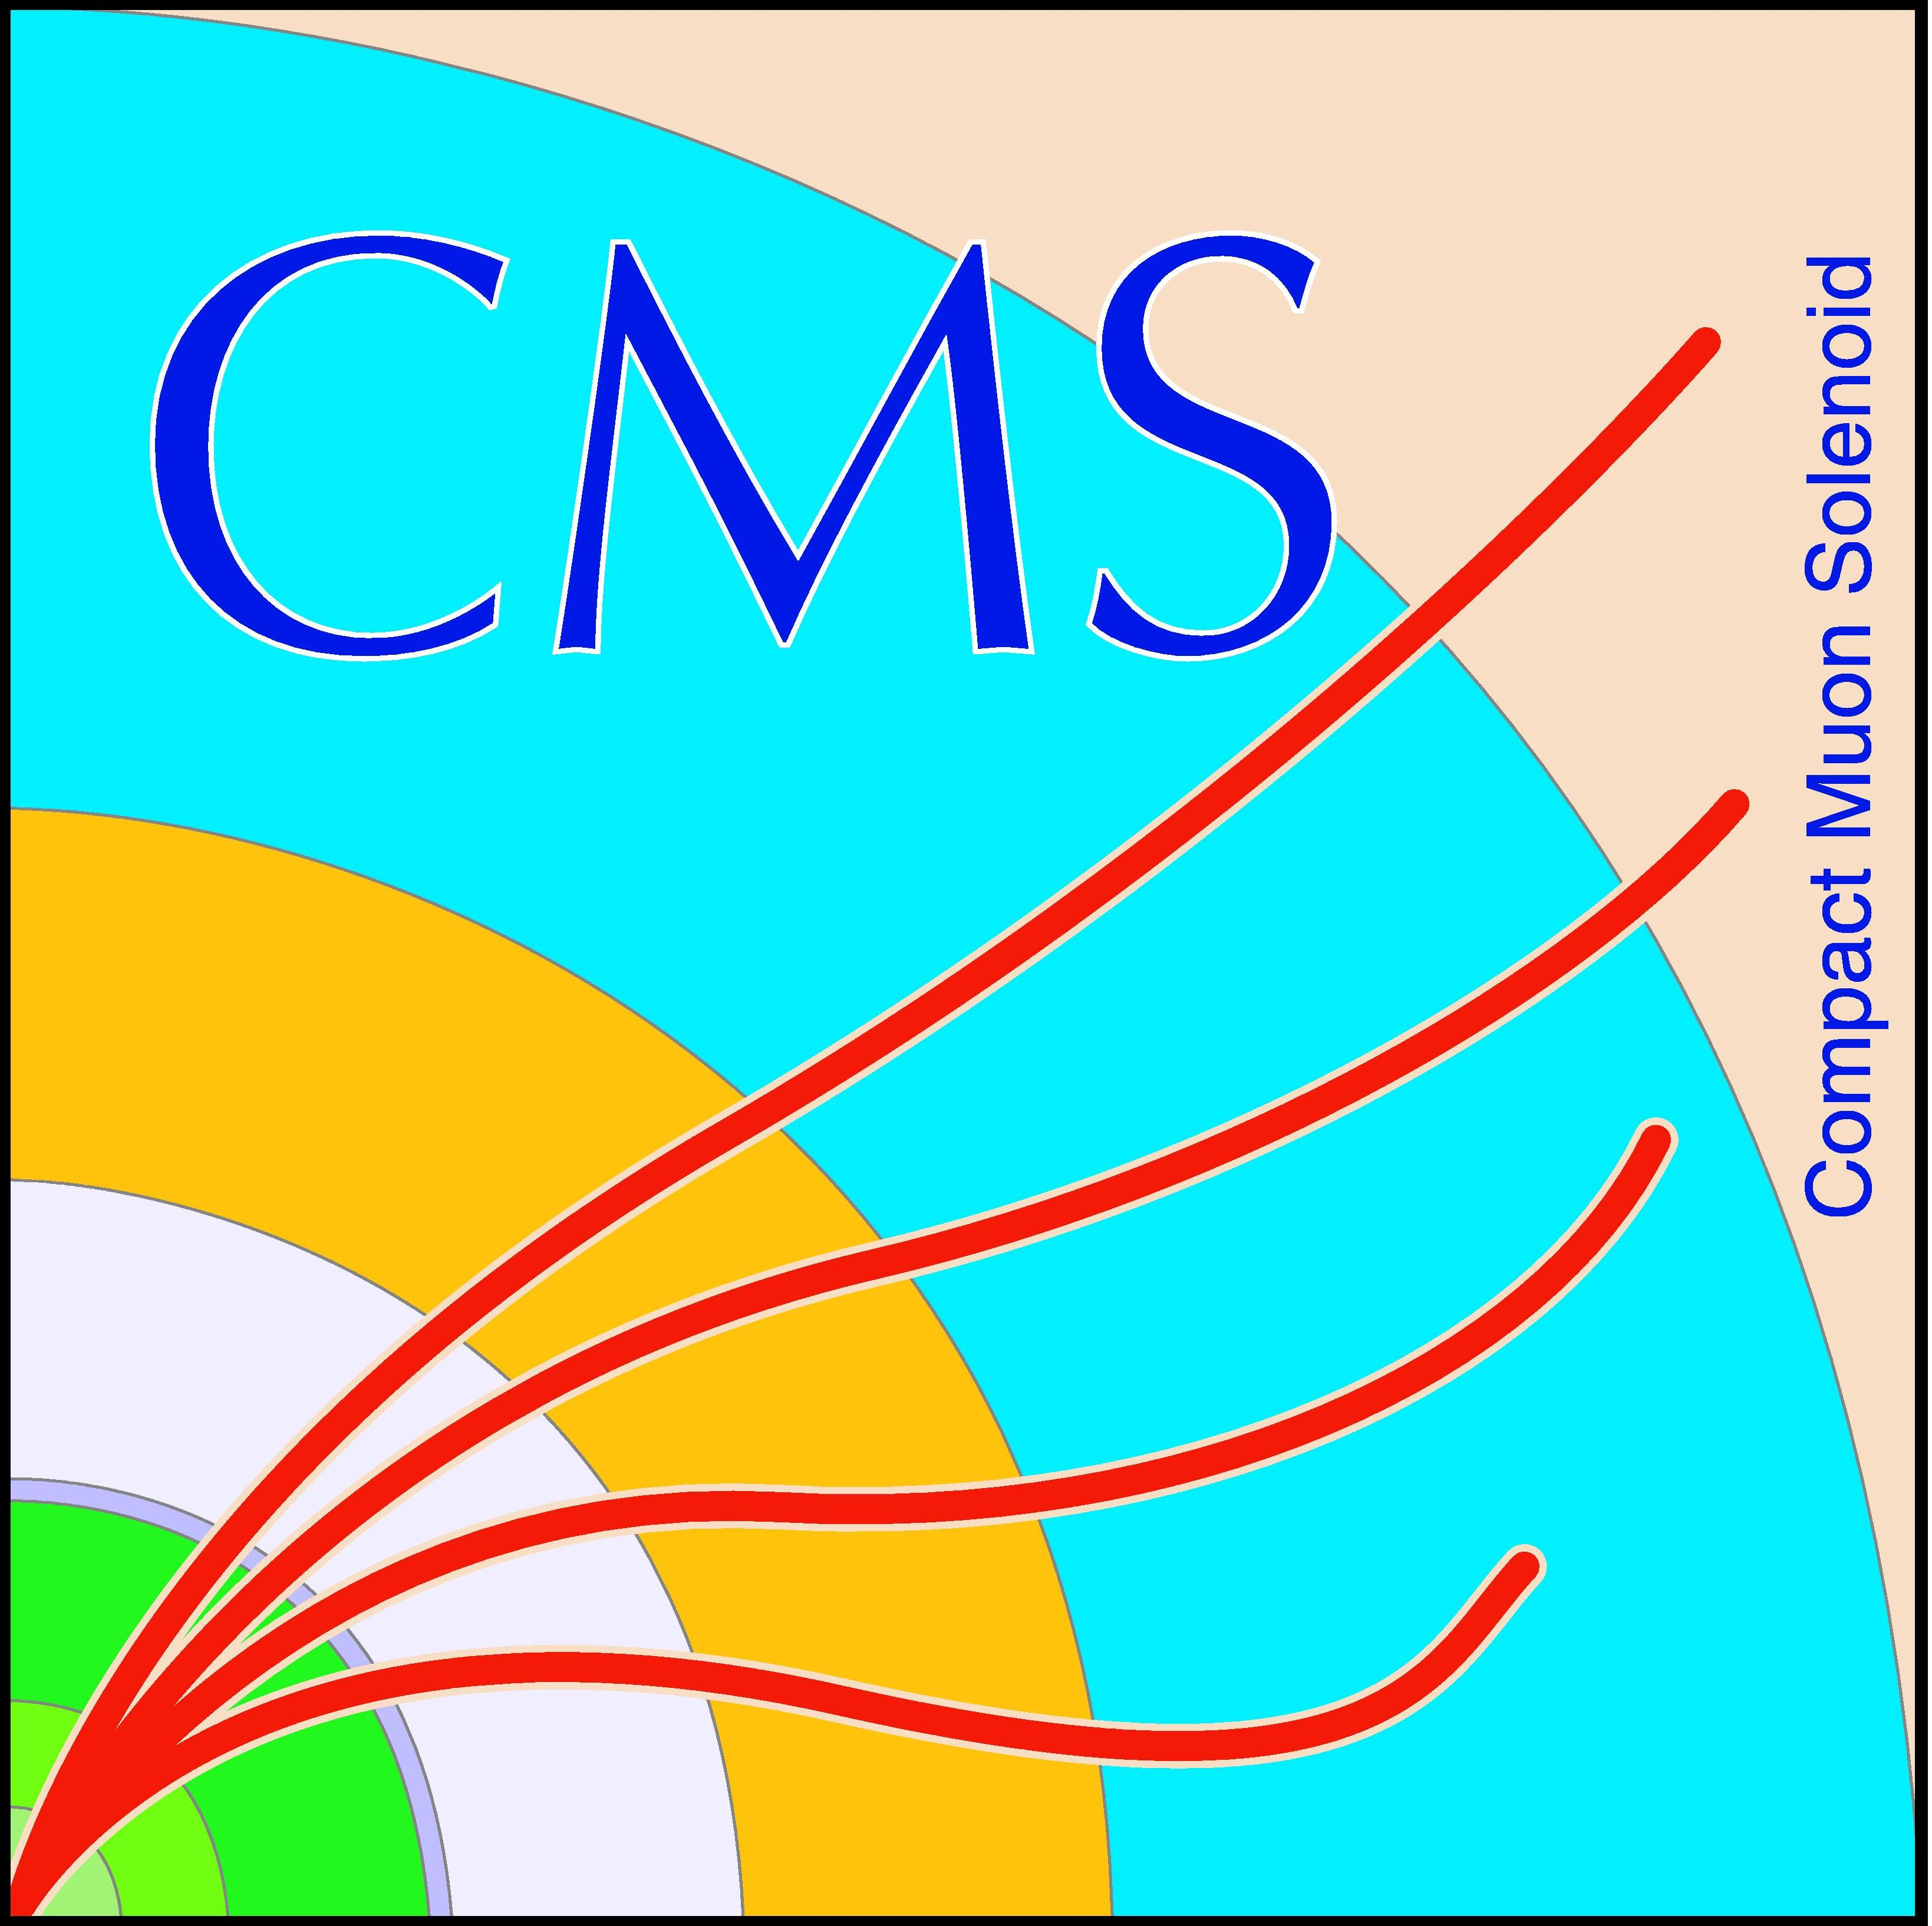
\includegraphics[height=1.5cm]{CMSlogo.jpeg}
  \end{center}
}

% pdflatex packages
\hypersetup{bookmarks=true}
\hypersetup{unicode=false}
\hypersetup{pdftitle={Islated Tracks}}
\hypersetup{pdfauthor={Arne-Rasmus~Dr\"ager}}


\begin{document}
% ==================================================
% --------------------------------------------------
\begin{frame}
  \titlepage
\end{frame}


% --------------------------------------------------

\section{Closure Studies}


\subsection{Efficiencies}
\begin{frame}
 \frametitle{Parametrization Problem}
 \begin{itemize}
  \item Previous choice of search variables as parametrization of lepton efficiencies good closure, but not ideal
  \begin{itemize}
   \item Not directly related to lepton properties
   \item Can not be derived from data $\rightarrow$ Need to rely on MC and use in different variables efficiencies from Tag and Probe for validation (delta R and rel \pt lepton to closest jet)
  \end{itemize}
  \item The former used delta R and rel \pt of lepton can not fully capture the kinematics because:
  \begin{itemize}
   \item Lost-leptons due to delta R in the range of isolation definition (0.3) of lepton have very small control sample (isolation criteria delta R \pt definition) which also means very low efficiency
   \item When going to low statistics search bins (a few single isolated leptons) statistics of small delta R (with low efficiency $\rightarrow$ high prediction) insufficient $\rightarrow$ underprediction
   \item Problematic for fine search binning!
  \end{itemize}
  \item When using 4D binned analysis either \BTags or \NJets show bad closure when using 3D binned lep efficiencies
 \end{itemize}
\end{frame}

\begin{frame}
 \frametitle{Solving Parametrization Problem: Idea}
 \begin{itemize}
  \item Try to move back to more lepton based parametrization of efficiencies
  \begin{itemize}
   \item Need to cope with low statistics and extension to 4D search binning
  \end{itemize}
  \item Approach:
  \begin{itemize}
   \item Define variable not orthogonal and not fully correlated with isolation criteria which captures the event kinematics in a broader spectrum than just the closest jet
   \item Define activity around lepton with relatively large cone $\Delta R=1.0$
  \end{itemize}
  \item Muon activity:
  \begin{itemize}
   \item $A = \sum_{Jet}^{\Delta R<1.0} \pt(Jet) * (ChargedEMFraction + ChargedHadFraction) $ 
  \end{itemize}
    \item Electron activity:
  \begin{itemize}
   \item $A = \sum_{Jet}^{\Delta R<1.0} \pt(Jet) * (ChargedHadFraction) $ 
  \end{itemize}
      \item IsoTrack activity:
  \begin{itemize}
   \item $A = \sum_{Jet}^{\Delta R<1.0} \pt(Jet) * (NeutralEMFraction + PhotonEFraction) $ 
  \end{itemize}
  \item Activity is strongly correlated to jet activity around lepton and with sum over large delta R captures event in broader perspective (helps at low stat regions!?)
 \end{itemize}
\end{frame}




\begin{frame}
\frametitle{Parametrization of Efficiencies}
  \begin{columns}
    \begin{column}{0.5\textwidth}
     \centering
     Old
     \begin{itemize}




        \item Isolation 
   \begin{itemize}
    \item \HT \MHT \NJets (\BTags)
   \end{itemize}
   \item Reconstruction 
   \begin{itemize}
    \item \HT \MHT \NJets (\BTags)
   \end{itemize}
   \item Acceptance 
   \begin{itemize}
    \item \MHT \NJets (\BTags)
   \end{itemize}
   \item Purity (only electron CS)
   \begin{itemize}
    \item \MHT \NJets 
   \end{itemize}
      \item Di-lep contamination
   \begin{itemize}
    \item \MHT \NJets 
   \end{itemize}
   \item Di-lep efficiency
   \begin{itemize}
    \item \NJets 
   \end{itemize}
   \item \mt cut efficiency
   \begin{itemize}
    \item \NJets 
   \end{itemize}
     \end{itemize}
    \end{column}
    \begin{column}{0.5\textwidth}
      \centering
      New
             \begin{itemize}


        \item Isolation 
   \begin{itemize}
    \item Lep \pt Activity
   \end{itemize}
   \item Reconstruction 
   \begin{itemize}
    \item Activity
   \end{itemize}
   \item Acceptance 
   \begin{itemize}
    \item \BTags \NJets
   \end{itemize}
   \item Purity (only electron CS)
   \begin{itemize}
    \item \MHT \NJets 
   \end{itemize}
      \item Di-lep contamination
   \begin{itemize}
    \item \NJets 
   \end{itemize}
   \item Di-lep efficiency
   \begin{itemize}
    \item \NJets 
   \end{itemize}
   \item \mt cut efficiency
   \begin{itemize}
    \item Activity 
   \end{itemize}
     \end{itemize}
    \end{column}
  \end{columns}
\end{frame}
\subsection{Closure}
\begin{frame}
 \begin{center}
    {\Large Closure Muon Control Sample}
  \end{center}
\end{frame}
\begin{frame}
\frametitle{Muon Control Sample: Closure Test \HT \& \MHT}
  \begin{columns}
    \begin{column}{0.5\textwidth}
     \centering
      \begin{overpic}[width=0.70\textwidth]{figures/Closure_Old_Parametrization/Closure__HT__MuPrMTWDiLep_vs_MCEx__Baseline.pdf}\put(100,60){\rotatebox{-90}{\scriptsize Old Parametrization Variables}}
     \end{overpic}
      \begin{overpic}[width=0.70\textwidth]{figures/Closure_Old_Parametrization/Closure__MHT__MuPrMTWDiLep_vs_MCEx__Baseline.pdf}
     \end{overpic}
    \end{column}
    \begin{column}{0.5\textwidth}
      \centering
      \begin{overpic}[width=0.70\textwidth]{figures/Closure_New_Parametrization/Closure__HT__MuPrMTWDiLep_vs_MCEx__Baseline.pdf} \put(100,60){\rotatebox{-90}{\scriptsize New Parametrization Variables}}     \end{overpic}
      \centering
      \begin{overpic}[width=0.70\textwidth]{figures/Closure_New_Parametrization/Closure__MHT__MuPrMTWDiLep_vs_MCEx__Baseline}     \end{overpic}
    \end{column}
  \end{columns}
\end{frame}

\begin{frame}
\frametitle{Muon Control Sample: Closure Test \NJets \& \BTags}
  \begin{columns}
    \begin{column}{0.5\textwidth}
     \centering
      \begin{overpic}[width=0.70\textwidth]{figures/Closure_Old_Parametrization/Closure__BTags__MuPrMTWDiLep_vs_MCEx__Baseline.pdf} \put(100,60){\rotatebox{-90}{\scriptsize Old Parametrization Variables}}
     \end{overpic}
      \begin{overpic}[width=0.70\textwidth]{figures/Closure_Old_Parametrization/Closure__NJets__MuPrMTWDiLep_vs_MCEx__Baseline.pdf}
     \end{overpic}
    \end{column}
    \begin{column}{0.5\textwidth}
      \centering
      \begin{overpic}[width=0.70\textwidth]{figures/Closure_New_Parametrization/Closure__BTags__MuPrMTWDiLep_vs_MCEx__Baseline.pdf}  \put(100,60){\rotatebox{-90}{\scriptsize New Parametrization Variables}}
      \end{overpic}
      \centering
      \begin{overpic}[width=0.70\textwidth]{figures/Closure_New_Parametrization/Closure__NJets__MuPrMTWDiLep_vs_MCEx__Baseline}     \end{overpic}
    \end{column}
  \end{columns}
\end{frame}

\begin{frame}
 \begin{center}
    {\Large Closure Eletron Control Sample}
  \end{center}
\end{frame}

\begin{frame}
\frametitle{Electron Control Sample: Closure Test \HT \& \MHT}
  \begin{columns}
    \begin{column}{0.5\textwidth}
     \centering
      \begin{overpic}[width=0.70\textwidth]{figures/Closure_Old_Parametrization/Closure__HT__ElecPrMTWDiLep_vs_MCEx__Baseline.pdf}\put(100,60){\rotatebox{-90}{\scriptsize Old Parametrization Variables}}
     \end{overpic}
      \begin{overpic}[width=0.70\textwidth]{figures/Closure_Old_Parametrization/Closure__MHT__ElecPrMTWDiLep_vs_MCEx__Baseline.pdf}
     \end{overpic}
    \end{column}
    \begin{column}{0.5\textwidth}
      \centering
      \begin{overpic}[width=0.70\textwidth]{figures/Closure_New_Parametrization/Closure__HT__ElecPrMTWDiLep_vs_MCEx__Baseline.pdf}  \put(100,60){\rotatebox{-90}{\scriptsize New Parametrization Variables}}   \end{overpic}
      \centering
      \begin{overpic}[width=0.70\textwidth]{figures/Closure_New_Parametrization/Closure__MHT__ElecPrMTWDiLep_vs_MCEx__Baseline}     \end{overpic}
    \end{column}
  \end{columns}
\end{frame}

\begin{frame}
\frametitle{Electron Control Sample Closure Test \NJets \& \BTags}
  \begin{columns}
    \begin{column}{0.5\textwidth}
     \centering
      \begin{overpic}[width=0.70\textwidth]{figures/Closure_Old_Parametrization/Closure__BTags__ElecPrMTWDiLep_vs_MCEx__Baseline.pdf} \put(100,60){\rotatebox{-90}{\scriptsize Old Parametrization Variables}}
     \end{overpic}
      \begin{overpic}[width=0.70\textwidth]{figures/Closure_Old_Parametrization/Closure__NJets__ElecPrMTWDiLep_vs_MCEx__Baseline.pdf}
     \end{overpic}
    \end{column}
    \begin{column}{0.5\textwidth}
      \centering
      \begin{overpic}[width=0.70\textwidth]{figures/Closure_New_Parametrization/Closure__BTags__ElecPrMTWDiLep_vs_MCEx__Baseline.pdf}  \put(100,60){\rotatebox{-90}{\scriptsize New Parametrization Variables}}   \end{overpic}
      \centering
      \begin{overpic}[width=0.70\textwidth]{figures/Closure_New_Parametrization/Closure__NJets__ElecPrMTWDiLep_vs_MCEx__Baseline}     \end{overpic}
    \end{column}
  \end{columns}
\end{frame}



\begin{frame}
 \begin{center}
    {\Large Combined Electron and Muon Control Sample Closure}
  \end{center}
\end{frame}
\begin{frame}
\frametitle{Muon \& Elec Control Sample Combined Closure}
  \begin{columns}
    \begin{column}{0.5\textwidth}
     \centering
      \begin{overpic}[width=0.70\textwidth]{figures/Closure_New_Parametrization/Closure_Combined__HT__MCEx_vs_MuPrMTWDiLep+ElecPrMTWDiLep__Baseline.pdf}
     \end{overpic}
     \begin{overpic}[width=0.70\textwidth]{figures/Closure_New_Parametrization/Closure_Combined__BTags__MCEx_vs_MuPrMTWDiLep+ElecPrMTWDiLep__Baseline.pdf}
     \end{overpic}
    \end{column}
    \begin{column}{0.5\textwidth}
      \centering
      \begin{overpic}[width=0.70\textwidth]{figures/Closure_New_Parametrization/Closure_Combined__MHT__MCEx_vs_MuPrMTWDiLep+ElecPrMTWDiLep__Baseline.pdf}     \end{overpic}
      \centering
      \begin{overpic}[width=0.70\textwidth]{figures/Closure_New_Parametrization/Closure_Combined__NJets__MCEx_vs_MuPrMTWDiLep+ElecPrMTWDiLep__Baseline.pdf}     \end{overpic}
    \end{column}
  \end{columns}
\end{frame}

\begin{frame}
 \begin{center}
    {\Large Separate Closure Muon Control Sample}
  \end{center}
\end{frame}

\subsection{Lost Lepton equations (reminder)}
\begin{frame}
 \begin{equation}
 \rm !ISO^{\mu} = {\rm CS}\cdot \frac{1-\epsilon_{\rm ISO}^{\mu}}{\epsilon_{\rm ISO}^{\mu}} 
    %%   \rm !ISO^{\mu}} = {\rm CS}\cdot \frac{1-\epsilon_{\rm ISO}^{\mu}}{\epsilon_{\rm ISO}^{\mu}} 
\label{eq:isolation_muon}
\end{equation}
\begin{equation}
 {\rm !Reco^{\mu}} = {\rm CS}\cdot \frac{1}{\epsilon_{\rm ISO}^{\mu}} \cdot \frac{1-\epsilon_{\rm Reco}^{\mu}}{\epsilon_{\rm Reco}^{\mu}}
\label{eq:reconstruction_muon}
\end{equation}
\begin{equation}
 {\rm !Acc^{\mu}} = {\rm CS}\cdot \frac{1}{\epsilon_{\rm ISO}^{\mu}}\cdot \frac{1}{\epsilon_{\rm Reco}^{\mu}} \cdot \frac{1-\epsilon^{\mu}_{Acc}}{\epsilon^{\mu}_{Acc}}
\label{eq:acceptance_muon}
\end{equation}
\begin{equation}
{\rm !Acc^{e}} = {\rm CS}\cdot \frac{1}{\epsilon_{\rm ISO}^{\mu}}\cdot \frac{1}{\epsilon_{\rm Reco}^{\mu}}  \cdot \frac{1 - \epsilon^{e}_{Acc}}{\epsilon^{\mu}_{Acc}}
 \label{eq:elec_acc}
\end{equation}
\begin{equation}
{\rm !Reco^{e}} = {\rm CS}\cdot \frac{1}{\epsilon_{\rm ISO}^{\mu}}\cdot \frac{1-\epsilon_{\rm Reco}^{e}}{\epsilon_{\rm Reco}^{\mu}}  \cdot \frac{\epsilon^{e}_{Acc}}{\epsilon^{\mu}_{Acc}}
 \label{eq:elec_reco}
\end{equation}
\begin{equation}
{\rm !ISO^{e}} = {\rm CS}\cdot \frac{1-\epsilon_{\rm ISO}^{e}}{\epsilon_{\rm ISO}^{\mu}} \cdot \frac{\epsilon^{e}_{Reco}}{\epsilon^{\mu}_{Reco}} \cdot \frac{\epsilon^{e}_{Acc}}{\epsilon^{\mu}_{Acc}}
\label{eq:elec_iso}
\end{equation}
\begin{itemize}
 \item Keep in mind the dependency of each step! Non-Closure propagates to all following precitions!
\end{itemize}

\end{frame}
\subsection{Muon CS Separate Closure}

\begin{frame}
 \frametitle{Muon Control Sample: Remaining Non-Closure $\mu$ Iso}
   \begin{columns}
    \begin{column}{0.5\textwidth}
     \centering
      \begin{overpic}[width=0.70\textwidth]{figures/separate_closure/Mu_Closure_test__HT__MuExIso_vs_MuCSPrIso__Baseline.pdf} 
     \end{overpic}
      \begin{overpic}[width=0.70\textwidth]{figures/separate_closure/Mu_Closure_test__BTags__MuExIso_vs_MuCSPrIso__Baseline.pdf} 
     \end{overpic}
    \end{column}
    \begin{column}{0.5\textwidth}
      \centering
      \begin{overpic}[width=0.70\textwidth]{figures/separate_closure/Mu_Closure_test__MHT__MuExIso_vs_MuCSPrIso__Baseline.pdf}     \end{overpic}
      \centering
      \begin{overpic}[width=0.70\textwidth]{figures/separate_closure/Mu_Closure_test__NJets__MuExIso_vs_MuCSPrIso__Baseline.pdf}     \end{overpic}
    \end{column}
  \end{columns}
\end{frame}
\begin{frame}
 \frametitle{Muon Control Sample: Remaining Non-Closure $\mu$ Reco}
   \begin{columns}
    \begin{column}{0.5\textwidth}
     \centering
      \begin{overpic}[width=0.70\textwidth]{figures/separate_closure/Mu_Closure_test__HT__MuExReco_vs_MuCSPrReco__Baseline.pdf} 
     \end{overpic}
      \begin{overpic}[width=0.70\textwidth]{figures/separate_closure/Mu_Closure_test__BTags__MuExReco_vs_MuCSPrReco__Baseline.pdf} 
     \end{overpic}
    \end{column}
    \begin{column}{0.5\textwidth}
      \centering
      \begin{overpic}[width=0.70\textwidth]{figures/separate_closure/Mu_Closure_test__MHT__MuExReco_vs_MuCSPrReco__Baseline.pdf}     \end{overpic}
      \centering
      \begin{overpic}[width=0.70\textwidth]{figures/separate_closure/Mu_Closure_test__NJets__MuExReco_vs_MuCSPrReco__Baseline.pdf}     \end{overpic}
    \end{column}
  \end{columns}
\end{frame}


\begin{frame}
 \frametitle{Muon Control Sample: Remaining Non-Closure $\mu$ Acc}
   \begin{columns}
    \begin{column}{0.5\textwidth}
     \centering
      \begin{overpic}[width=0.70\textwidth]{figures/separate_closure/Mu_Closure_test__HT__MuExAcc_vs_MuCSPrAcc__Baseline.pdf} 
     \end{overpic}
      \begin{overpic}[width=0.70\textwidth]{figures/separate_closure/Mu_Closure_test__BTags__MuExAcc_vs_MuCSPrAcc__Baseline.pdf} 
     \end{overpic}
    \end{column}
    \begin{column}{0.5\textwidth}
      \centering
      \begin{overpic}[width=0.70\textwidth]{figures/separate_closure/Mu_Closure_test__MHT__MuExAcc_vs_MuCSPrAcc__Baseline.pdf}     \end{overpic}
      \centering
      \begin{overpic}[width=0.70\textwidth]{figures/separate_closure/Mu_Closure_test__NJets__MuExAcc_vs_MuCSPrAcc__Baseline.pdf}     \end{overpic}
    \end{column}
  \end{columns}
\end{frame}


\begin{frame}
 \frametitle{Muon Control Sample: Remaining Non-Closure e Acc}
   \begin{columns}
    \begin{column}{0.5\textwidth}
     \centering
      \begin{overpic}[width=0.70\textwidth]{figures/separate_closure/Elec_Closure_test__HT__ElecExAcc_vs_MuCSPrAcc__Baseline.pdf} 
     \end{overpic}
      \begin{overpic}[width=0.70\textwidth]{figures/separate_closure/Elec_Closure_test__BTags__ElecExAcc_vs_MuCSPrAcc__Baseline.pdf} 
     \end{overpic}
    \end{column}
    \begin{column}{0.5\textwidth}
      \centering
      \begin{overpic}[width=0.70\textwidth]{figures/separate_closure/Elec_Closure_test__MHT__ElecExAcc_vs_MuCSPrAcc__Baseline.pdf}     \end{overpic}
      \centering
      \begin{overpic}[width=0.70\textwidth]{figures/separate_closure/Elec_Closure_test__NJets__ElecExAcc_vs_MuCSPrAcc__Baseline.pdf}     \end{overpic}
    \end{column}
  \end{columns}
\end{frame}


\begin{frame}
 \frametitle{Muon Control Sample: Remaining Non-Closure e Reco}
   \begin{columns}
    \begin{column}{0.5\textwidth}
     \centering
      \begin{overpic}[width=0.70\textwidth]{figures/separate_closure/Elec_Closure_test__HT__ElecExReco_vs_MuCSPrReco__Baseline.pdf} 
     \end{overpic}
      \begin{overpic}[width=0.70\textwidth]{figures/separate_closure/Elec_Closure_test__BTags__ElecExReco_vs_MuCSPrReco__Baseline.pdf} 
     \end{overpic}
    \end{column}
    \begin{column}{0.5\textwidth}
      \centering
      \begin{overpic}[width=0.70\textwidth]{figures/separate_closure/Elec_Closure_test__MHT__ElecExReco_vs_MuCSPrReco__Baseline.pdf}     \end{overpic}
      \centering
      \begin{overpic}[width=0.70\textwidth]{figures/separate_closure/Elec_Closure_test__NJets__ElecExReco_vs_MuCSPrReco__Baseline.pdf}     \end{overpic}
    \end{column}
  \end{columns}
\end{frame}


\begin{frame}
 \frametitle{Muon Control Sample: Remaining Non-Closure e Iso}
   \begin{columns}
    \begin{column}{0.5\textwidth}
     \centering
      \begin{overpic}[width=0.70\textwidth]{figures/separate_closure/Elec_Closure_test__HT__ElecExIso_vs_MuCSPrIso__Baseline.pdf} 
     \end{overpic}
      \begin{overpic}[width=0.70\textwidth]{figures/separate_closure/Elec_Closure_test__BTags__ElecExIso_vs_MuCSPrIso__Baseline.pdf} 
     \end{overpic}
    \end{column}
    \begin{column}{0.5\textwidth}
      \centering
      \begin{overpic}[width=0.70\textwidth]{figures/separate_closure/Elec_Closure_test__MHT__ElecExIso_vs_MuCSPrIso__Baseline.pdf}     \end{overpic}
      \centering
      \begin{overpic}[width=0.70\textwidth]{figures/separate_closure/Elec_Closure_test__NJets__ElecExIso_vs_MuCSPrIso__Baseline.pdf}     \end{overpic}
    \end{column}
  \end{columns}
\end{frame}

\subsection{Electron CS Separate Closure}
\begin{frame}
 \begin{center}
    {\Large Separate Closure Eletron Control Sample}
  \end{center}
\end{frame}


\begin{frame}
 \frametitle{Elec Control Sample: Remaining Non-Closure e Iso}
   \begin{columns}
    \begin{column}{0.5\textwidth}
     \centering
      \begin{overpic}[width=0.70\textwidth]{figures/separate_closure/Elec_Closure_test__HT__ElecExIso_vs_ElecCSPrIso__Baseline.pdf} 
     \end{overpic}
      \begin{overpic}[width=0.70\textwidth]{figures/separate_closure/Elec_Closure_test__BTags__ElecExIso_vs_ElecCSPrIso__Baseline.pdf} 
     \end{overpic}
    \end{column}
    \begin{column}{0.5\textwidth}
      \centering
      \begin{overpic}[width=0.70\textwidth]{figures/separate_closure/Elec_Closure_test__MHT__ElecExIso_vs_ElecCSPrIso__Baseline.pdf}     \end{overpic}
      \centering
      \begin{overpic}[width=0.70\textwidth]{figures/separate_closure/Elec_Closure_test__NJets__ElecExIso_vs_ElecCSPrIso__Baseline.pdf}     \end{overpic}
    \end{column}
  \end{columns}
\end{frame}



\begin{frame}
 \frametitle{Elec Control Sample: Remaining Non-Closure e Reco}
   \begin{columns}
    \begin{column}{0.5\textwidth}
     \centering
      \begin{overpic}[width=0.70\textwidth]{figures/separate_closure/Elec_Closure_test__HT__ElecExReco_vs_ElecCSPrReco__Baseline.pdf} 
     \end{overpic}
      \begin{overpic}[width=0.70\textwidth]{figures/separate_closure/Elec_Closure_test__BTags__ElecExReco_vs_ElecCSPrReco__Baseline.pdf} 
     \end{overpic}
    \end{column}
    \begin{column}{0.5\textwidth}
      \centering
      \begin{overpic}[width=0.70\textwidth]{figures/separate_closure/Elec_Closure_test__MHT__ElecExReco_vs_ElecCSPrReco__Baseline.pdf}     \end{overpic}
      \centering
      \begin{overpic}[width=0.70\textwidth]{figures/separate_closure/Elec_Closure_test__NJets__ElecExReco_vs_ElecCSPrReco__Baseline.pdf}     \end{overpic}
    \end{column}
  \end{columns}
\end{frame}





\begin{frame}
 \frametitle{Elec Control Sample: Remaining Non-Closure e Acc}
   \begin{columns}
    \begin{column}{0.5\textwidth}
     \centering
      \begin{overpic}[width=0.70\textwidth]{figures/separate_closure/Elec_Closure_test__HT__ElecExAcc_vs_ElecCSPrAcc__Baseline.pdf} 
     \end{overpic}
      \begin{overpic}[width=0.70\textwidth]{figures/separate_closure/Elec_Closure_test__BTags__ElecExAcc_vs_ElecCSPrAcc__Baseline.pdf} 
     \end{overpic}
    \end{column}
    \begin{column}{0.5\textwidth}
      \centering
      \begin{overpic}[width=0.70\textwidth]{figures/separate_closure/Elec_Closure_test__MHT__ElecExAcc_vs_ElecCSPrAcc__Baseline.pdf}     \end{overpic}
      \centering
      \begin{overpic}[width=0.70\textwidth]{figures/separate_closure/Elec_Closure_test__NJets__ElecExAcc_vs_ElecCSPrAcc__Baseline.pdf}     \end{overpic}
    \end{column}
  \end{columns}
\end{frame}


\begin{frame}
 \frametitle{Elec Control Sample: Remaining Non-Closure $\mu$ Acc}
   \begin{columns}
    \begin{column}{0.5\textwidth}
     \centering
      \begin{overpic}[width=0.70\textwidth]{figures/separate_closure/Mu_Closure_test__HT__MuExAcc_vs_ElecCSPrAcc__Baseline.pdf} 
     \end{overpic}
      \begin{overpic}[width=0.70\textwidth]{figures/separate_closure/Mu_Closure_test__BTags__MuExAcc_vs_ElecCSPrAcc__Baseline.pdf} 
     \end{overpic}
    \end{column}
    \begin{column}{0.5\textwidth}
      \centering
      \begin{overpic}[width=0.70\textwidth]{figures/separate_closure/Mu_Closure_test__MHT__MuExAcc_vs_ElecCSPrAcc__Baseline.pdf}     \end{overpic}
      \centering
      \begin{overpic}[width=0.70\textwidth]{figures/separate_closure/Mu_Closure_test__NJets__MuExAcc_vs_ElecCSPrAcc__Baseline.pdf}     \end{overpic}
    \end{column}
  \end{columns}
\end{frame}




\begin{frame}
 \frametitle{Elec Control Sample: Remaining Non-Closure $\mu$ Reco}
   \begin{columns}
    \begin{column}{0.5\textwidth}
     \centering
      \begin{overpic}[width=0.70\textwidth]{figures/separate_closure/Mu_Closure_test__HT__MuExReco_vs_ElecCSPrReco__Baseline.pdf} 
     \end{overpic}
      \begin{overpic}[width=0.70\textwidth]{figures/separate_closure/Mu_Closure_test__BTags__MuExReco_vs_ElecCSPrReco__Baseline.pdf} 
     \end{overpic}
    \end{column}
    \begin{column}{0.5\textwidth}
      \centering
      \begin{overpic}[width=0.70\textwidth]{figures/separate_closure/Mu_Closure_test__MHT__MuExReco_vs_ElecCSPrReco__Baseline.pdf}     \end{overpic}
      \centering
      \begin{overpic}[width=0.70\textwidth]{figures/separate_closure/Mu_Closure_test__NJets__MuExReco_vs_ElecCSPrReco__Baseline.pdf}     \end{overpic}
    \end{column}
  \end{columns}
\end{frame}



\begin{frame}
 \frametitle{Elec Control Sample: Remaining Non-Closure $\mu$ Iso}
   \begin{columns}
    \begin{column}{0.5\textwidth}
     \centering
      \begin{overpic}[width=0.70\textwidth]{figures/separate_closure/Mu_Closure_test__HT__MuExIso_vs_ElecCSPrIso__Baseline.pdf} 
     \end{overpic}
      \begin{overpic}[width=0.70\textwidth]{figures/separate_closure/Mu_Closure_test__BTags__MuExIso_vs_ElecCSPrIso__Baseline.pdf} 
     \end{overpic}
    \end{column}
    \begin{column}{0.5\textwidth}
      \centering
      \begin{overpic}[width=0.70\textwidth]{figures/separate_closure/Mu_Closure_test__MHT__MuExIso_vs_ElecCSPrIso__Baseline.pdf}     \end{overpic}
      \centering
      \begin{overpic}[width=0.70\textwidth]{figures/separate_closure/Mu_Closure_test__NJets__MuExIso_vs_ElecCSPrIso__Baseline.pdf}     \end{overpic}
    \end{column}
  \end{columns}
\end{frame}

\subsection{Muon Efficiencies}
\begin{frame}
 \begin{center}
    {\Large Efficiencies: Muon}
  \end{center}
\end{frame}

\begin{frame}
\frametitle{$\mu$ iso}
   \begin{columns}
    \begin{column}{0.33\textwidth}
     \centering
      \begin{overpic}[width=1.00\textwidth]{figures/efficiencies/MuIsoHT1D.pdf} 
     \end{overpic}
      \begin{overpic}[width=1.00\textwidth]{figures/efficiencies/MuIsoNJets1D.pdf} 
     \end{overpic}
    \end{column}
    \begin{column}{0.33\textwidth}
      \centering
      \begin{overpic}[width=1.00\textwidth]{figures/efficiencies/MuIsoMHT1D.pdf}      \end{overpic}
      \centering
      \begin{overpic}[width=1.00\textwidth]{figures/efficiencies/MuIsoPT.pdf}      \end{overpic}
    \end{column}
    \begin{column}{0.33\textwidth}
     \centering
      \begin{overpic}[width=1.00\textwidth]{figures/efficiencies/MuIsoBTag1D.pdf}      \end{overpic}
      \begin{overpic}[width=1.00\textwidth]{figures/efficiencies/MuIsoActivity.pdf} \end{overpic}

    \end{column}

  \end{columns}
\end{frame}

\begin{frame}
 \frametitle{$\mu$ iso used parametization and binnning}
\centering
      \begin{overpic}[width=0.90\textwidth]{figures/efficiencies/MuIsoPTActivity.pdf} 
     \end{overpic}
\end{frame}

\begin{frame}
\frametitle{$\mu$ reco}
   \begin{columns}
    \begin{column}{0.33\textwidth}
     \centering
      \begin{overpic}[width=1.00\textwidth]{figures/efficiencies/MuRecoHT1D.pdf} 
     \end{overpic}
      \begin{overpic}[width=1.00\textwidth]{figures/efficiencies/MuRecoNJets1D.pdf} 
     \end{overpic}
    \end{column}
    \begin{column}{0.33\textwidth}
      \centering
      \begin{overpic}[width=1.00\textwidth]{figures/efficiencies/MuRecoMHT1D.pdf}      \end{overpic}
      \centering
      \begin{overpic}[width=1.00\textwidth]{figures/efficiencies/MuRecoPT.pdf}      \end{overpic}
    \end{column}
    \begin{column}{0.33\textwidth}
     \centering
      \begin{overpic}[width=1.00\textwidth]{figures/efficiencies/MuRecoBTag1D.pdf}      \end{overpic}
         \begin{overpic}[width=1.00\textwidth]{figures/efficiencies/MuRecoActivity.pdf} \end{overpic}

    \end{column}

  \end{columns}
\end{frame}

\begin{frame}
 \frametitle{$\mu$ reco used parametization and binnning}
\centering
      \begin{overpic}[width=0.90\textwidth]{figures/efficiencies/MuRecoActivity.pdf} 
     \end{overpic}
\end{frame}

\begin{frame}
\frametitle{$\mu$ acc}
   \begin{columns}
    \begin{column}{0.33\textwidth}
     \centering
      \begin{overpic}[width=1.00\textwidth]{figures/efficiencies/MuAccHT1D.pdf} 
     \end{overpic}
      \begin{overpic}[width=1.00\textwidth]{figures/efficiencies/MuAccNJets1D.pdf} 
     \end{overpic}
    \end{column}
    \begin{column}{0.33\textwidth}
      \centering
      \begin{overpic}[width=1.00\textwidth]{figures/efficiencies/MuAccMHT1D.pdf}      \end{overpic}
      \begin{overpic}[width=1.00\textwidth]{figures/efficiencies/MuAccActivity.pdf} \end{overpic}
      \centering
    \end{column}
    \begin{column}{0.33\textwidth}
     \centering
      \begin{overpic}[width=1.00\textwidth]{figures/efficiencies/MuAccBTag1D.pdf}      \end{overpic}
\begin{overpic}[width=1.00\textwidth]{figures/efficiencies/MuAccPT.pdf}      \end{overpic}

    \end{column}

  \end{columns}
\end{frame}

\begin{frame}
 \frametitle{$\mu$ acc used parametization and binnning}
\centering
      \begin{overpic}[width=0.90\textwidth]{figures/efficiencies/MuAccBTagNJets.pdf} 
     \end{overpic}
\end{frame}

\begin{frame}
\frametitle{$\mu$ Purity}
   \begin{columns}
    \begin{column}{0.33\textwidth}
     \centering
      \begin{overpic}[width=1.00\textwidth]{figures/efficiencies/MuPurityHT1D.pdf} 
     \end{overpic}
      \begin{overpic}[width=1.00\textwidth]{figures/efficiencies/MuPurityNJets1D.pdf} 
     \end{overpic}
    \end{column}
    \begin{column}{0.33\textwidth}
      \centering
      \begin{overpic}[width=1.00\textwidth]{figures/efficiencies/MuPurityMHT1D.pdf}      \end{overpic}
      \begin{overpic}[width=1.00\textwidth]{figures/efficiencies/MuPurityActivity.pdf} \end{overpic}
      \centering
    \end{column}
    \begin{column}{0.33\textwidth}
     \centering
      \begin{overpic}[width=1.00\textwidth]{figures/efficiencies/MuPurityBTag1D.pdf}      \end{overpic}
\begin{overpic}[width=1.00\textwidth]{figures/efficiencies/MuPurityPT.pdf}      \end{overpic}

    \end{column}

  \end{columns}
\end{frame}


\begin{frame}
 \begin{center}
    {\Large $\mu$ purity not corrected for!}
  \end{center}
\end{frame}

\begin{frame}
\frametitle{$\mu$ \mt-cut}
   \begin{columns}
    \begin{column}{0.33\textwidth}
     \centering
      \begin{overpic}[width=1.00\textwidth]{figures/efficiencies/MuMTWHT1D.pdf} 
     \end{overpic}
      \begin{overpic}[width=1.00\textwidth]{figures/efficiencies/MuMTWNJets1D.pdf} 
     \end{overpic}
    \end{column}
    \begin{column}{0.33\textwidth}
      \centering
      \begin{overpic}[width=1.00\textwidth]{figures/efficiencies/MuMTWMHT1D.pdf}      \end{overpic}
      \begin{overpic}[width=1.00\textwidth]{figures/efficiencies/MuMTWActivity.pdf} \end{overpic}
      \centering
    \end{column}
    \begin{column}{0.33\textwidth}
     \centering
      \begin{overpic}[width=1.00\textwidth]{figures/efficiencies/MuMTWBTag1D.pdf}      \end{overpic}
\begin{overpic}[width=1.00\textwidth]{figures/efficiencies/MuMTWPT.pdf}      \end{overpic}

    \end{column}

  \end{columns}
\end{frame}


\begin{frame}
 \frametitle{$\mu$ \mt-cut used parametization and binnning}
\centering
      \begin{overpic}[width=0.90\textwidth]{figures/efficiencies/MuMTWPTActivity.pdf} 
     \end{overpic}
\end{frame}


\begin{frame}
\frametitle{$\mu$ di lep contribution to control sample}
   \begin{columns}
    \begin{column}{0.33\textwidth}
     \centering
      \begin{overpic}[width=1.00\textwidth]{figures/efficiencies/MuDiLepContributionHT1D.pdf} 
     \end{overpic}
      \begin{overpic}[width=1.00\textwidth]{figures/efficiencies/MuDiLepContributionNJets1D.pdf} 
     \end{overpic}
    \end{column}
    \begin{column}{0.33\textwidth}
      \centering
      \begin{overpic}[width=1.00\textwidth]{figures/efficiencies/MuDiLepContributionMHT1D.pdf}      \end{overpic}
            \begin{overpic}[width=1.00\textwidth]{figures/efficiencies/MuDiLepContributionBTag1D.pdf}      \end{overpic}
      \centering
    \end{column}
  \end{columns}
\end{frame}


\begin{frame}
 \frametitle{$\mu$ di lep contamination used parametization and binnning}
\centering
      \begin{overpic}[width=1.00\textwidth]{figures/efficiencies/MuDiLepContributionNJets1D.pdf} 
     \end{overpic}
\end{frame}



\subsection{Electron Efficiencies}
\begin{frame}
 \begin{center}
    {\Large Efficiencies: Electron}
  \end{center}
\end{frame}

\begin{frame}
\frametitle{e iso}
   \begin{columns}
    \begin{column}{0.33\textwidth}
     \centering
      \begin{overpic}[width=1.00\textwidth]{figures/efficiencies/ElecIsoHT1D.pdf} 
     \end{overpic}
      \begin{overpic}[width=1.00\textwidth]{figures/efficiencies/ElecIsoNJets1D.pdf} 
     \end{overpic}
    \end{column}
    \begin{column}{0.33\textwidth}
      \centering
      \begin{overpic}[width=1.00\textwidth]{figures/efficiencies/ElecIsoMHT1D.pdf}      \end{overpic}
      \centering
      \begin{overpic}[width=1.00\textwidth]{figures/efficiencies/ElecIsoPT.pdf}      \end{overpic}
    \end{column}
    \begin{column}{0.33\textwidth}
     \centering
      \begin{overpic}[width=1.00\textwidth]{figures/efficiencies/ElecIsoBTag1D.pdf}      \end{overpic}
      \begin{overpic}[width=1.00\textwidth]{figures/efficiencies/ElecIsoActivity.pdf} \end{overpic}

    \end{column}

  \end{columns}
\end{frame}

\begin{frame}
 \frametitle{e iso used parametization and binnning}
\centering
      \begin{overpic}[width=0.90\textwidth]{figures/efficiencies/ElecIsoPTActivity.pdf} 
     \end{overpic}
\end{frame}

\begin{frame}
\frametitle{e reco}
   \begin{columns}
    \begin{column}{0.33\textwidth}
     \centering
      \begin{overpic}[width=1.00\textwidth]{figures/efficiencies/ElecRecoHT1D.pdf} 
     \end{overpic}
      \begin{overpic}[width=1.00\textwidth]{figures/efficiencies/ElecRecoNJets1D.pdf} 
     \end{overpic}
    \end{column}
    \begin{column}{0.33\textwidth}
      \centering
      \begin{overpic}[width=1.00\textwidth]{figures/efficiencies/ElecRecoMHT1D.pdf}      \end{overpic}
      \centering
      \begin{overpic}[width=1.00\textwidth]{figures/efficiencies/ElecRecoPT.pdf}      \end{overpic}
    \end{column}
    \begin{column}{0.33\textwidth}
     \centering
      \begin{overpic}[width=1.00\textwidth]{figures/efficiencies/ElecRecoBTag1D.pdf}      \end{overpic}
         \begin{overpic}[width=1.00\textwidth]{figures/efficiencies/ElecRecoActivity.pdf} \end{overpic}

    \end{column}

  \end{columns}
\end{frame}

\begin{frame}
 \frametitle{e reco used parametization and binnning}
\centering
      \begin{overpic}[width=0.90\textwidth]{figures/efficiencies/ElecRecoActivity.pdf} 
     \end{overpic}
\end{frame}

\begin{frame}
\frametitle{e acc}
   \begin{columns}
    \begin{column}{0.33\textwidth}
     \centering
      \begin{overpic}[width=1.00\textwidth]{figures/efficiencies/ElecAccHT1D.pdf} 
     \end{overpic}
      \begin{overpic}[width=1.00\textwidth]{figures/efficiencies/ElecAccNJets1D.pdf} 
     \end{overpic}
    \end{column}
    \begin{column}{0.33\textwidth}
      \centering
      \begin{overpic}[width=1.00\textwidth]{figures/efficiencies/ElecAccMHT1D.pdf}      \end{overpic}
      \begin{overpic}[width=1.00\textwidth]{figures/efficiencies/ElecAccActivity.pdf} \end{overpic}
      \centering
    \end{column}
    \begin{column}{0.33\textwidth}
     \centering
      \begin{overpic}[width=1.00\textwidth]{figures/efficiencies/ElecAccBTag1D.pdf}      \end{overpic}
\begin{overpic}[width=1.00\textwidth]{figures/efficiencies/ElecAccPT.pdf}      \end{overpic}

    \end{column}

  \end{columns}
\end{frame}

\begin{frame}
 \frametitle{e acc used parametization and binnning}
\centering
      \begin{overpic}[width=0.90\textwidth]{figures/efficiencies/ElecAccBTagNJets.pdf} 
     \end{overpic}
\end{frame}

\begin{frame}
\frametitle{e Purity}
   \begin{columns}
    \begin{column}{0.33\textwidth}
     \centering
      \begin{overpic}[width=1.00\textwidth]{figures/efficiencies/ElecPurityHT1D.pdf} 
     \end{overpic}
      \begin{overpic}[width=1.00\textwidth]{figures/efficiencies/ElecPurityNJets1D.pdf} 
     \end{overpic}
    \end{column}
    \begin{column}{0.33\textwidth}
      \centering
      \begin{overpic}[width=1.00\textwidth]{figures/efficiencies/ElecPurityMHT1D.pdf}      \end{overpic}
      \begin{overpic}[width=1.00\textwidth]{figures/efficiencies/ElecPurityActivity.pdf} \end{overpic}
      \centering
    \end{column}
    \begin{column}{0.33\textwidth}
     \centering
      \begin{overpic}[width=1.00\textwidth]{figures/efficiencies/ElecPurityBTag1D.pdf}      \end{overpic}
\begin{overpic}[width=1.00\textwidth]{figures/efficiencies/ElecPurityPT.pdf}      \end{overpic}

    \end{column}

  \end{columns}
\end{frame}


\begin{frame}
 \frametitle{e purity used parametization and binnning}
\centering
      \begin{overpic}[width=0.90\textwidth]{figures/efficiencies/ElecPurity.pdf} 
     \end{overpic}
\end{frame}

\begin{frame}
\frametitle{e \mt-cut}
   \begin{columns}
    \begin{column}{0.33\textwidth}
     \centering
      \begin{overpic}[width=1.00\textwidth]{figures/efficiencies/ElecMTWHT1D.pdf} 
     \end{overpic}
      \begin{overpic}[width=1.00\textwidth]{figures/efficiencies/ElecMTWNJets1D.pdf} 
     \end{overpic}
    \end{column}
    \begin{column}{0.33\textwidth}
      \centering
      \begin{overpic}[width=1.00\textwidth]{figures/efficiencies/ElecMTWMHT1D.pdf}      \end{overpic}
      \begin{overpic}[width=1.00\textwidth]{figures/efficiencies/ElecMTWActivity.pdf} \end{overpic}
      \centering
    \end{column}
    \begin{column}{0.33\textwidth}
     \centering
      \begin{overpic}[width=1.00\textwidth]{figures/efficiencies/ElecMTWBTag1D.pdf}      \end{overpic}
\begin{overpic}[width=1.00\textwidth]{figures/efficiencies/ElecMTWPT.pdf}      \end{overpic}

    \end{column}

  \end{columns}
\end{frame}


\begin{frame}
 \frametitle{e \mt-cut used parametization and binnning}
\centering
      \begin{overpic}[width=0.90\textwidth]{figures/efficiencies/ElecMTWPTActivity.pdf} 
     \end{overpic}
\end{frame}


\begin{frame}
\frametitle{e di lep contribution to control sample}
   \begin{columns}
    \begin{column}{0.33\textwidth}
     \centering
      \begin{overpic}[width=1.00\textwidth]{figures/efficiencies/ElecDiLepContributionHT1D.pdf} 
     \end{overpic}
      \begin{overpic}[width=1.00\textwidth]{figures/efficiencies/ElecDiLepContributionNJets1D.pdf} 
     \end{overpic}
    \end{column}
    \begin{column}{0.33\textwidth}
      \centering
      \begin{overpic}[width=1.00\textwidth]{figures/efficiencies/ElecDiLepContributionMHT1D.pdf}      \end{overpic}
            \begin{overpic}[width=1.00\textwidth]{figures/efficiencies/ElecDiLepContributionBTag1D.pdf}      \end{overpic}
      \centering
    \end{column}
  \end{columns}
\end{frame}


\begin{frame}
 \frametitle{e di lep contribution used parametization and binnning}
\centering
      \begin{overpic}[width=1.00\textwidth]{figures/efficiencies/ElecDiLepContributionNJets1D.pdf} 
     \end{overpic}
\end{frame}

\subsection{Closure Search bins}
\begin{frame}
 \begin{center}
    {\Large Closure for fine search bins of\\ \HT, \MHT, \NJets \& \BTags}
  \end{center}
\end{frame}
\begin{frame}
\tiny
\begin{tabular}{lrrrr}
\toprule

                                                Selection  &                     MCEx  &           ElecPr  &             MuPr  &          Combined Pre.  \\ 
\midrule
     BTag\_0\_NJet\_3-5\_\_HT\_0500-0800\_\_MHT\_200-300 &             $888.4\pm7.9$&             $413.4\pm4.6$&             $429.8\pm5.1$&                $843.2\pm11.5$ \\ 
      BTag\_0\_NJet\_3-5\_\_HT\_0500-0800\_\_MHT\_300-450 &             $335.9\pm4.6$&             $159.8\pm2.5$&             $165.5\pm2.8$&                 $325.3\pm6.2$ \\ 
      BTag\_0\_NJet\_3-5\_\_HT\_0500-0800\_\_MHT\_450-600 &              $65.6\pm1.8$&              $27.8\pm0.9$&              $29.3\pm1.0$&                  $57.2\pm2.2$ \\ 
      BTag\_0\_NJet\_3-5\_\_HT\_0500-0800\_\_MHT\_600-Inf &               $7.8\pm0.5$&               $2.6\pm0.2$&               $3.0\pm0.2$&                   $5.6\pm0.4$ \\ 
      BTag\_0\_NJet\_3-5\_\_HT\_0800-1000\_\_MHT\_200-300 &             $132.1\pm2.6$&              $67.5\pm1.8$&              $65.4\pm1.7$&                 $132.8\pm4.3$ \\ 
      BTag\_0\_NJet\_3-5\_\_HT\_0800-1000\_\_MHT\_300-450 &              $57.2\pm1.6$&              $30.0\pm1.0$&              $31.1\pm1.1$&                  $61.1\pm2.5$ \\ 
      BTag\_0\_NJet\_3-5\_\_HT\_0800-1000\_\_MHT\_450-600 &              $17.0\pm0.8$&               $9.1\pm0.5$&              $10.7\pm0.6$&                  $19.8\pm1.3$ \\ 
      BTag\_0\_NJet\_3-5\_\_HT\_0800-1000\_\_MHT\_600-Inf &               $8.8\pm0.6$&               $4.3\pm0.3$&               $4.3\pm0.3$&                   $8.6\pm0.8$ \\ 
      BTag\_0\_NJet\_3-5\_\_HT\_1000-1250\_\_MHT\_200-300 &              $56.8\pm1.6$&              $28.1\pm1.0$&              $30.3\pm1.3$&                  $58.3\pm2.6$ \\ 
      BTag\_0\_NJet\_3-5\_\_HT\_1000-1250\_\_MHT\_300-450 &              $25.3\pm1.1$&              $14.2\pm0.6$&              $16.1\pm0.9$&                  $30.3\pm1.7$ \\ 
      BTag\_0\_NJet\_3-5\_\_HT\_1000-1250\_\_MHT\_450-600 &               $7.7\pm0.6$&               $4.6\pm0.4$&               $4.7\pm0.4$&                   $9.4\pm0.9$ \\ 
      BTag\_0\_NJet\_3-5\_\_HT\_1000-1250\_\_MHT\_600-Inf &               $5.3\pm0.4$&               $2.9\pm0.2$&               $2.9\pm0.3$&                   $5.8\pm0.6$ \\ 
      BTag\_0\_NJet\_3-5\_\_HT\_1250-1500\_\_MHT\_200-300 &              $19.9\pm0.9$&               $9.2\pm0.5$&              $10.1\pm0.6$&                  $19.3\pm1.3$ \\ 
      BTag\_0\_NJet\_3-5\_\_HT\_1250-1500\_\_MHT\_300-450 &               $7.8\pm0.5$&               $5.3\pm0.4$&               $5.7\pm0.4$&                  $11.1\pm0.9$ \\ 
      BTag\_0\_NJet\_3-5\_\_HT\_1250-1500\_\_MHT\_450-Inf &               $5.0\pm0.5$&               $3.3\pm0.3$&               $3.3\pm0.3$&                   $6.6\pm0.7$ \\ 
       BTag\_0\_NJet\_3-5\_\_HT\_1500-Inf\_\_MHT\_200-300 &              $14.0\pm0.8$&               $6.9\pm0.5$&               $7.0\pm0.5$&                  $13.9\pm1.2$ \\ 
       BTag\_0\_NJet\_3-5\_\_HT\_1500-Inf\_\_MHT\_300-Inf &              $11.7\pm0.7$&               $6.3\pm0.4$&               $6.3\pm0.4$&                  $12.6\pm1.0$ \\ 
      BTag\_0\_NJet\_6-7\_\_HT\_0500-0800\_\_MHT\_200-300 &              $41.8\pm2.4$&              $21.1\pm1.2$&              $20.1\pm1.3$&                  $41.2\pm3.1$ \\ 
      BTag\_0\_NJet\_6-7\_\_HT\_0500-0800\_\_MHT\_300-450 &               $9.2\pm1.0$&               $4.6\pm0.6$&               $4.0\pm0.6$&                   $8.6\pm1.5$ \\ 
      BTag\_0\_NJet\_6-7\_\_HT\_0500-0800\_\_MHT\_450-Inf &               $0.6\pm0.2$&               $0.2\pm0.0$&               $0.3\pm0.2$&                   $0.5\pm0.2$ \\ 
      BTag\_0\_NJet\_6-7\_\_HT\_0800-1000\_\_MHT\_200-300 &              $18.6\pm1.4$&              $11.0\pm0.9$&               $9.5\pm0.9$&                  $20.4\pm2.2$ \\ 
      BTag\_0\_NJet\_6-7\_\_HT\_0800-1000\_\_MHT\_300-450 &               $5.3\pm0.7$&               $3.5\pm0.4$&               $3.3\pm0.4$&                   $6.8\pm1.0$ \\ 
      BTag\_0\_NJet\_6-7\_\_HT\_0800-1000\_\_MHT\_450-Inf &               $1.3\pm0.3$&               $0.6\pm0.1$&               $0.7\pm0.2$&                   $1.3\pm0.4$ \\ 
      BTag\_0\_NJet\_6-7\_\_HT\_1000-1250\_\_MHT\_200-300 &              $10.8\pm1.0$&               $6.4\pm0.7$&               $5.6\pm0.6$&                  $12.0\pm1.6$ \\ 
      BTag\_0\_NJet\_6-7\_\_HT\_1000-1250\_\_MHT\_300-450 &               $5.0\pm0.7$&               $2.4\pm0.3$&               $3.5\pm0.5$&                   $5.9\pm0.9$ \\ 
      BTag\_0\_NJet\_6-7\_\_HT\_1000-1250\_\_MHT\_450-Inf &               $1.1\pm0.3$&               $0.8\pm0.1$&               $0.8\pm0.2$&                   $1.6\pm0.4$ \\ 
      BTag\_0\_NJet\_6-7\_\_HT\_1250-1500\_\_MHT\_200-300 &               $4.2\pm0.6$&               $2.4\pm0.4$&               $2.6\pm0.3$&                   $5.1\pm0.9$ \\ 
      BTag\_0\_NJet\_6-7\_\_HT\_1250-1500\_\_MHT\_300-450 &               $2.2\pm0.4$&               $1.6\pm0.3$&               $1.1\pm0.3$&                   $2.7\pm0.8$ \\ 
      BTag\_0\_NJet\_6-7\_\_HT\_1250-1500\_\_MHT\_450-Inf &               $0.7\pm0.2$&               $0.7\pm0.1$&               $0.6\pm0.2$&                   $1.3\pm0.4$ \\ 
       BTag\_0\_NJet\_6-7\_\_HT\_1500-Inf\_\_MHT\_200-300 &               $4.6\pm0.6$&               $2.0\pm0.3$&               $1.8\pm0.3$&                   $3.8\pm0.8$ \\ 
       BTag\_0\_NJet\_6-7\_\_HT\_1500-Inf\_\_MHT\_300-Inf &               $2.4\pm0.4$&               $2.2\pm0.4$&               $1.6\pm0.3$&                   $3.9\pm0.8$ \\ 
    BTag\_0\_NJet\_8-Inf\_\_HT\_0500-0800\_\_MHT\_200-Inf &               $0.6\pm0.3$&               $0.6\pm0.2$&               $0.5\pm0.2$&                   $1.1\pm0.5$ \\ 
    BTag\_0\_NJet\_8-Inf\_\_HT\_0800-1000\_\_MHT\_200-Inf &               $1.4\pm0.4$&               $1.0\pm0.3$&               $1.3\pm0.3$&                   $2.3\pm0.7$ \\ 
    BTag\_0\_NJet\_8-Inf\_\_HT\_1000-1250\_\_MHT\_200-Inf &               $1.6\pm0.5$&               $1.1\pm0.3$&               $0.6\pm0.2$&                   $1.6\pm0.7$ \\ 
    BTag\_0\_NJet\_8-Inf\_\_HT\_1250-1500\_\_MHT\_200-Inf &               $1.0\pm0.3$&               $0.3\pm0.1$&               $0.9\pm0.3$&                   $1.1\pm0.4$ \\ 
     BTag\_0\_NJet\_8-Inf\_\_HT\_1500-Inf\_\_MHT\_200-Inf &               $1.0\pm0.3$&               $0.6\pm0.2$&               $1.4\pm0.4$&                   $2.0\pm0.6$ \\ 

\bottomrule 
\end{tabular}
\end{frame}

\begin{frame}
\tiny
\begin{tabular}{lrrrr}
\toprule

                                                Selection  &                     MCEx  &           ElecPr  &             MuPr  &          Combined Pre.  \\ 
\midrule
       BTag\_1\_NJet\_3-5\_\_HT\_0500-0800\_\_MHT\_200-300 &             $609.3\pm9.1$&             $276.2\pm5.3$&             $293.5\pm6.3$&                $569.7\pm13.6$ \\ 
      BTag\_1\_NJet\_3-5\_\_HT\_0500-0800\_\_MHT\_300-450 &             $184.4\pm4.9$&              $80.4\pm2.7$&              $83.8\pm3.2$&                 $164.2\pm6.9$ \\ 
      BTag\_1\_NJet\_3-5\_\_HT\_0500-0800\_\_MHT\_450-600 &              $22.4\pm1.5$&              $10.4\pm0.9$&              $10.8\pm1.1$&                  $21.2\pm2.3$ \\ 
      BTag\_1\_NJet\_3-5\_\_HT\_0500-0800\_\_MHT\_600-Inf &               $2.0\pm0.4$&               $0.9\pm0.2$&               $0.7\pm0.2$&                   $1.6\pm0.5$ \\ 
      BTag\_1\_NJet\_3-5\_\_HT\_0800-1000\_\_MHT\_200-300 &              $93.9\pm3.5$&              $38.5\pm2.0$&              $36.8\pm2.2$&                  $75.3\pm5.0$ \\ 
      BTag\_1\_NJet\_3-5\_\_HT\_0800-1000\_\_MHT\_300-450 &              $33.8\pm2.0$&              $17.0\pm1.3$&              $14.0\pm1.2$&                  $31.0\pm3.0$ \\ 
      BTag\_1\_NJet\_3-5\_\_HT\_0800-1000\_\_MHT\_450-600 &               $7.5\pm0.9$&               $4.3\pm0.6$&               $3.9\pm0.7$&                   $8.2\pm1.6$ \\ 
      BTag\_1\_NJet\_3-5\_\_HT\_0800-1000\_\_MHT\_600-Inf &               $2.7\pm0.5$&               $1.1\pm0.2$&               $1.0\pm0.2$&                   $2.1\pm0.5$ \\ 
      BTag\_1\_NJet\_3-5\_\_HT\_1000-1250\_\_MHT\_200-300 &              $39.8\pm2.2$&              $19.0\pm1.5$&              $17.4\pm1.5$&                  $36.3\pm3.5$ \\ 
      BTag\_1\_NJet\_3-5\_\_HT\_1000-1250\_\_MHT\_300-450 &              $15.7\pm1.4$&               $8.9\pm0.9$&               $6.3\pm1.0$&                  $15.2\pm2.3$ \\ 
      BTag\_1\_NJet\_3-5\_\_HT\_1000-1250\_\_MHT\_450-600 &               $3.2\pm0.6$&               $1.7\pm0.3$&               $1.7\pm0.3$&                   $3.4\pm0.8$ \\ 
      BTag\_1\_NJet\_3-5\_\_HT\_1000-1250\_\_MHT\_600-Inf &               $2.0\pm0.4$&               $1.0\pm0.2$&               $0.7\pm0.2$&                   $1.8\pm0.5$ \\ 
      BTag\_1\_NJet\_3-5\_\_HT\_1250-1500\_\_MHT\_200-300 &              $11.4\pm1.1$&               $5.6\pm0.8$&               $5.1\pm0.8$&                  $10.8\pm1.9$ \\ 
      BTag\_1\_NJet\_3-5\_\_HT\_1250-1500\_\_MHT\_300-450 &               $5.4\pm0.8$&               $2.2\pm0.4$&               $3.4\pm0.7$&                   $5.6\pm1.3$ \\ 
      BTag\_1\_NJet\_3-5\_\_HT\_1250-1500\_\_MHT\_450-Inf &               $2.2\pm0.4$&               $1.0\pm0.2$&               $1.2\pm0.4$&                   $2.2\pm0.7$ \\ 
       BTag\_1\_NJet\_3-5\_\_HT\_1500-Inf\_\_MHT\_200-300 &               $7.7\pm0.9$&               $2.8\pm0.5$&               $3.8\pm0.7$&                   $6.6\pm1.4$ \\ 
       BTag\_1\_NJet\_3-5\_\_HT\_1500-Inf\_\_MHT\_300-Inf &               $6.4\pm0.8$&               $3.0\pm0.5$&               $2.4\pm0.5$&                   $5.4\pm1.2$ \\ 
      BTag\_1\_NJet\_6-7\_\_HT\_0500-0800\_\_MHT\_200-300 &              $70.0\pm3.3$&              $38.9\pm1.9$&              $33.8\pm2.0$&                  $72.7\pm4.6$ \\ 
      BTag\_1\_NJet\_6-7\_\_HT\_0500-0800\_\_MHT\_300-450 &              $12.1\pm1.3$&               $6.1\pm0.7$&               $7.3\pm1.0$&                  $13.4\pm1.9$ \\ 
      BTag\_1\_NJet\_6-7\_\_HT\_0500-0800\_\_MHT\_450-Inf &               $1.1\pm0.4$&               $0.1\pm0.1$&               $0.3\pm0.2$&                   $0.4\pm0.3$ \\ 
      BTag\_1\_NJet\_6-7\_\_HT\_0800-1000\_\_MHT\_200-300 &              $30.6\pm2.1$&              $17.8\pm1.4$&              $18.9\pm1.6$&                  $36.7\pm3.5$ \\ 
      BTag\_1\_NJet\_6-7\_\_HT\_0800-1000\_\_MHT\_300-450 &               $8.2\pm1.1$&               $6.4\pm0.8$&               $3.5\pm0.6$&                   $9.9\pm1.9$ \\ 
      BTag\_1\_NJet\_6-7\_\_HT\_0800-1000\_\_MHT\_450-Inf &               $1.2\pm0.4$&               $0.8\pm0.2$&               $1.4\pm0.5$&                   $2.2\pm0.8$ \\ 
      BTag\_1\_NJet\_6-7\_\_HT\_1000-1250\_\_MHT\_200-300 &              $20.9\pm1.8$&              $11.5\pm1.1$&              $11.0\pm1.3$&                  $22.4\pm2.9$ \\ 
      BTag\_1\_NJet\_6-7\_\_HT\_1000-1250\_\_MHT\_300-450 &               $7.3\pm1.0$&               $4.4\pm0.7$&               $3.0\pm0.5$&                   $7.4\pm1.5$ \\ 
      BTag\_1\_NJet\_6-7\_\_HT\_1000-1250\_\_MHT\_450-Inf &               $2.8\pm0.6$&               $0.9\pm0.2$&               $0.4\pm0.1$&                   $1.3\pm0.5$ \\ 
      BTag\_1\_NJet\_6-7\_\_HT\_1250-1500\_\_MHT\_200-300 &               $7.3\pm1.0$&               $3.5\pm0.6$&               $3.4\pm0.7$&                   $6.9\pm1.6$ \\ 
      BTag\_1\_NJet\_6-7\_\_HT\_1250-1500\_\_MHT\_300-450 &               $2.6\pm0.6$&               $1.6\pm0.4$&               $2.1\pm0.5$&                   $3.6\pm1.0$ \\ 
      BTag\_1\_NJet\_6-7\_\_HT\_1250-1500\_\_MHT\_450-Inf &               $1.1\pm0.4$&               $0.6\pm0.2$&               $0.7\pm0.3$&                   $1.3\pm0.6$ \\ 
       BTag\_1\_NJet\_6-7\_\_HT\_1500-Inf\_\_MHT\_200-300 &               $4.5\pm0.8$&               $3.3\pm0.6$&               $3.7\pm0.8$&                   $7.0\pm1.6$ \\ 
       BTag\_1\_NJet\_6-7\_\_HT\_1500-Inf\_\_MHT\_300-Inf &               $4.0\pm0.7$&               $2.4\pm0.5$&               $2.3\pm0.5$&                   $4.7\pm1.2$ \\ 
    BTag\_1\_NJet\_8-Inf\_\_HT\_0500-0800\_\_MHT\_200-Inf &               $3.2\pm0.7$&               $1.0\pm0.3$&               $0.5\pm0.2$&                   $1.5\pm0.6$ \\ 
    BTag\_1\_NJet\_8-Inf\_\_HT\_0800-1000\_\_MHT\_200-Inf &               $3.7\pm0.7$&               $2.1\pm0.4$&               $1.7\pm0.5$&                   $3.7\pm1.0$ \\ 
    BTag\_1\_NJet\_8-Inf\_\_HT\_1000-1250\_\_MHT\_200-Inf &               $4.4\pm0.8$&               $2.1\pm0.4$&               $2.6\pm0.6$&                   $4.7\pm1.2$ \\ 
    BTag\_1\_NJet\_8-Inf\_\_HT\_1250-1500\_\_MHT\_200-Inf &               $2.3\pm0.6$&               $1.9\pm0.5$&               $1.2\pm0.3$&                   $3.0\pm1.1$ \\ 
     BTag\_1\_NJet\_8-Inf\_\_HT\_1500-Inf\_\_MHT\_200-Inf &               $2.6\pm0.6$&               $1.4\pm0.4$&               $1.9\pm0.5$&                   $3.3\pm1.0$ \\ 

\bottomrule 
\end{tabular}
\end{frame}

\begin{frame}
\tiny
\begin{tabular}{lrrrr}
\toprule

                                                Selection  &                     MCEx  &           ElecPr  &             MuPr  &          Combined Pre.  \\ 
\midrule
  BTag\_2\_Inf\_NJet\_3-5\_\_HT\_0500-0800\_\_MHT\_200-300 &             $345.0\pm7.3$&             $167.3\pm4.7$&             $158.3\pm5.1$&                $325.6\pm11.6$ \\ 
 BTag\_2\_Inf\_NJet\_3-5\_\_HT\_0500-0800\_\_MHT\_300-450 &              $95.4\pm3.8$&              $40.0\pm2.3$&              $34.2\pm2.3$&                  $74.2\pm5.5$ \\ 
 BTag\_2\_Inf\_NJet\_3-5\_\_HT\_0500-0800\_\_MHT\_450-600 &               $7.3\pm1.0$&               $4.3\pm0.7$&               $3.3\pm0.8$&                   $7.6\pm1.8$ \\ 
 BTag\_2\_Inf\_NJet\_3-5\_\_HT\_0500-0800\_\_MHT\_600-Inf &               $0.1\pm0.1$&               $0.1\pm0.0$&               $0.1\pm0.1$&                   $0.2\pm0.1$ \\ 
 BTag\_2\_Inf\_NJet\_3-5\_\_HT\_0800-1000\_\_MHT\_200-300 &              $53.7\pm2.9$&              $22.9\pm1.8$&              $24.6\pm2.1$&                  $47.6\pm4.6$ \\ 
 BTag\_2\_Inf\_NJet\_3-5\_\_HT\_0800-1000\_\_MHT\_300-450 &              $17.2\pm1.6$&              $10.7\pm1.2$&               $8.8\pm1.3$&                  $19.5\pm3.0$ \\ 
 BTag\_2\_Inf\_NJet\_3-5\_\_HT\_0800-1000\_\_MHT\_450-600 &               $3.8\pm0.7$&               $2.6\pm0.6$&               $2.2\pm0.6$&                   $4.8\pm1.5$ \\ 
 BTag\_2\_Inf\_NJet\_3-5\_\_HT\_0800-1000\_\_MHT\_600-Inf &               $1.1\pm0.4$&               $0.4\pm0.2$&               $0.4\pm0.3$&                   $0.9\pm0.6$ \\ 
 BTag\_2\_Inf\_NJet\_3-5\_\_HT\_1000-1250\_\_MHT\_200-300 &              $20.0\pm1.7$&               $8.8\pm1.1$&               $9.4\pm1.3$&                  $18.2\pm2.9$ \\ 
 BTag\_2\_Inf\_NJet\_3-5\_\_HT\_1000-1250\_\_MHT\_300-450 &               $8.4\pm1.1$&               $5.2\pm0.9$&               $3.7\pm0.8$&                   $9.0\pm2.1$ \\ 
 BTag\_2\_Inf\_NJet\_3-5\_\_HT\_1000-1250\_\_MHT\_450-600 &               $2.3\pm0.6$&               $0.6\pm0.3$&               $1.2\pm0.5$&                   $1.8\pm0.8$ \\ 
 BTag\_2\_Inf\_NJet\_3-5\_\_HT\_1000-1250\_\_MHT\_600-Inf &               $0.8\pm0.3$&               $0.4\pm0.2$&               $0.4\pm0.3$&                   $0.8\pm0.5$ \\ 
 BTag\_2\_Inf\_NJet\_3-5\_\_HT\_1250-1500\_\_MHT\_200-300 &               $5.6\pm0.9$&               $2.4\pm0.6$&               $3.1\pm0.8$&                   $5.5\pm1.6$ \\ 
 BTag\_2\_Inf\_NJet\_3-5\_\_HT\_1250-1500\_\_MHT\_300-450 &               $3.7\pm0.8$&               $1.5\pm0.5$&               $1.0\pm0.4$&                   $2.5\pm1.2$ \\ 
 BTag\_2\_Inf\_NJet\_3-5\_\_HT\_1250-1500\_\_MHT\_450-Inf &               $1.1\pm0.4$&               $0.4\pm0.2$&               $0.8\pm0.4$&                   $1.2\pm0.6$ \\ 
  BTag\_2\_Inf\_NJet\_3-5\_\_HT\_1500-Inf\_\_MHT\_200-300 &               $4.8\pm0.8$&               $1.8\pm0.5$&               $1.8\pm0.6$&                   $3.6\pm1.3$ \\ 
  BTag\_2\_Inf\_NJet\_3-5\_\_HT\_1500-Inf\_\_MHT\_300-Inf &               $2.2\pm0.6$&               $1.0\pm0.4$&               $1.0\pm0.4$&                   $2.0\pm0.9$ \\ 
 BTag\_2\_Inf\_NJet\_6-7\_\_HT\_0500-0800\_\_MHT\_200-300 &              $68.0\pm3.3$&              $35.7\pm1.9$&              $33.3\pm2.1$&                  $69.0\pm4.7$ \\ 
 BTag\_2\_Inf\_NJet\_6-7\_\_HT\_0500-0800\_\_MHT\_300-450 &              $10.5\pm1.3$&               $5.4\pm0.8$&               $5.8\pm0.9$&                  $11.2\pm1.9$ \\ 
 BTag\_2\_Inf\_NJet\_6-7\_\_HT\_0500-0800\_\_MHT\_450-Inf &               $0.7\pm0.3$&               $0.4\pm0.3$&               $0.4\pm0.3$&                   $0.8\pm0.7$ \\ 
 BTag\_2\_Inf\_NJet\_6-7\_\_HT\_0800-1000\_\_MHT\_200-300 &              $31.2\pm2.2$&              $19.2\pm1.5$&              $17.6\pm1.5$&                  $36.8\pm3.6$ \\ 
 BTag\_2\_Inf\_NJet\_6-7\_\_HT\_0800-1000\_\_MHT\_300-450 &               $8.8\pm1.2$&               $6.0\pm0.8$&               $3.8\pm0.7$&                   $9.8\pm1.9$ \\ 
 BTag\_2\_Inf\_NJet\_6-7\_\_HT\_0800-1000\_\_MHT\_450-Inf &               $1.3\pm0.5$&               $0.4\pm0.2$&               $0.2\pm0.1$&                   $0.7\pm0.4$ \\ 
 BTag\_2\_Inf\_NJet\_6-7\_\_HT\_1000-1250\_\_MHT\_200-300 &              $18.6\pm1.7$&              $10.9\pm1.2$&               $8.5\pm1.1$&                  $19.5\pm2.8$ \\ 
 BTag\_2\_Inf\_NJet\_6-7\_\_HT\_1000-1250\_\_MHT\_300-450 &               $8.3\pm1.1$&               $3.5\pm0.6$&               $2.4\pm0.6$&                   $5.9\pm1.5$ \\ 
 BTag\_2\_Inf\_NJet\_6-7\_\_HT\_1000-1250\_\_MHT\_450-Inf &               $1.1\pm0.4$&               $0.7\pm0.3$&               $0.6\pm0.3$&                   $1.3\pm0.7$ \\ 
 BTag\_2\_Inf\_NJet\_6-7\_\_HT\_1250-1500\_\_MHT\_200-300 &               $7.8\pm1.1$&               $3.9\pm0.7$&               $2.9\pm0.7$&                   $6.8\pm1.7$ \\ 
 BTag\_2\_Inf\_NJet\_6-7\_\_HT\_1250-1500\_\_MHT\_300-450 &               $3.4\pm0.7$&               $2.1\pm0.6$&               $1.5\pm0.5$&                   $3.5\pm1.3$ \\ 
 BTag\_2\_Inf\_NJet\_6-7\_\_HT\_1250-1500\_\_MHT\_450-Inf &               $1.3\pm0.5$&               $0.5\pm0.3$&               $0.4\pm0.2$&                   $0.9\pm0.6$ \\ 
  BTag\_2\_Inf\_NJet\_6-7\_\_HT\_1500-Inf\_\_MHT\_200-300 &               $5.1\pm0.9$&               $3.0\pm0.7$&               $2.7\pm0.7$&                   $5.7\pm1.6$ \\ 
  BTag\_2\_Inf\_NJet\_6-7\_\_HT\_1500-Inf\_\_MHT\_300-Inf &               $2.9\pm0.7$&               $0.8\pm0.3$&               $0.7\pm0.3$&                   $1.4\pm0.7$ \\ 
 BTag\_2\_Inf\_NJet\_8-Inf\_\_HT\_0500-0800\_\_MHT\_200-Inf &               $1.8\pm0.5$&               $0.6\pm0.3$&               $0.9\pm0.3$&                   $1.5\pm0.7$ \\ 
 BTag\_2\_Inf\_NJet\_8-Inf\_\_HT\_0800-1000\_\_MHT\_200-Inf &               $4.1\pm0.8$&               $2.6\pm0.5$&               $3.7\pm0.8$&                   $6.3\pm1.4$ \\ 
 BTag\_2\_Inf\_NJet\_8-Inf\_\_HT\_1000-1250\_\_MHT\_200-Inf &               $5.6\pm0.9$&               $3.2\pm0.6$&               $3.3\pm0.6$&                   $6.5\pm1.4$ \\ 
 BTag\_2\_Inf\_NJet\_8-Inf\_\_HT\_1250-1500\_\_MHT\_200-Inf &               $1.2\pm0.4$&               $2.3\pm0.5$&               $2.1\pm0.6$&                   $4.3\pm1.3$ \\ 
 BTag\_2\_Inf\_NJet\_8-Inf\_\_HT\_1500-Inf\_\_MHT\_200-Inf &               $3.0\pm0.7$&               $1.9\pm0.5$&               $1.8\pm0.5$&                   $3.7\pm1.3$ \\ 

\bottomrule 
\end{tabular}
\end{frame}





% --------------------------------------------------
% --------------------------------------------------
\section{Conclusion}
\begin{frame}
 \begin{itemize}
 \item Problem with parametrization following either \NJets or \BTags search bin definition can be improved by using more lepton relevant based variables
 \item Updated parametrization of isolation, reconstruction, \mt-cut and di-lep contribution using \pt and activity around lepton shows reasonable closure for all search variables
 \item Further improvement and studies necessary. Especially non-closure in \NJets arising from out of acceptance leptons can be further improved
 \item Closure test for each of the 100 search bins needs to be studied!
 \item Work on extension of method using isolated tracks ongoing
 \end{itemize}

\end{frame}


\section{Backup}
\begin{frame}
  \begin{center}
    {\Large Additional Material}
  \end{center}
\end{frame}

% --------------------------------------------------

\subsection{ControlSamples}
\begin{frame}
\tiny
\begin{tabular}{lrrr}
\toprule

                                                Selection  &                   ElecCS  &                     MuCS  &          Total MC Control Sample  \\ 
\midrule
                                             Baseline &           $3296.0\pm18.4$&           $2941.4\pm17.2$&               $6237.4\pm43.6$ \\ 
      BTag\_0\_NJet\_3-5\_\_HT\_0500-0800\_\_MHT\_200-300 &             $661.9\pm6.8$&             $627.6\pm6.7$&               $1289.5\pm16.4$ \\ 
      BTag\_0\_NJet\_3-5\_\_HT\_0500-0800\_\_MHT\_300-450 &             $281.5\pm4.0$&             $265.3\pm3.9$&                 $546.9\pm9.6$ \\ 
      BTag\_0\_NJet\_3-5\_\_HT\_0500-0800\_\_MHT\_450-600 &              $50.4\pm1.4$&              $48.6\pm1.3$&                  $99.0\pm3.3$ \\ 
      BTag\_0\_NJet\_3-5\_\_HT\_0500-0800\_\_MHT\_600-Inf &               $4.9\pm0.3$&               $5.1\pm0.4$&                  $10.0\pm0.8$ \\ 
      BTag\_0\_NJet\_3-5\_\_HT\_0800-1000\_\_MHT\_200-300 &              $90.9\pm2.0$&              $83.2\pm1.9$&                 $174.0\pm4.8$ \\ 
      BTag\_0\_NJet\_3-5\_\_HT\_0800-1000\_\_MHT\_300-450 &              $46.5\pm1.4$&              $44.1\pm1.2$&                  $90.5\pm3.2$ \\ 
      BTag\_0\_NJet\_3-5\_\_HT\_0800-1000\_\_MHT\_450-600 &              $15.7\pm0.7$&              $16.2\pm0.8$&                  $31.8\pm1.8$ \\ 
      BTag\_0\_NJet\_3-5\_\_HT\_0800-1000\_\_MHT\_600-Inf &               $7.7\pm0.4$&               $7.8\pm0.5$&                  $15.4\pm1.1$ \\ 
      BTag\_0\_NJet\_3-5\_\_HT\_1000-1250\_\_MHT\_200-300 &              $37.7\pm1.2$&              $34.1\pm1.0$&                  $71.8\pm2.8$ \\ 
      BTag\_0\_NJet\_3-5\_\_HT\_1000-1250\_\_MHT\_300-450 &              $20.6\pm0.9$&              $20.7\pm0.9$&                  $41.3\pm2.1$ \\ 
      BTag\_0\_NJet\_3-5\_\_HT\_1000-1250\_\_MHT\_450-600 &               $7.5\pm0.5$&               $6.8\pm0.5$&                  $14.4\pm1.2$ \\ 
      BTag\_0\_NJet\_3-5\_\_HT\_1000-1250\_\_MHT\_600-Inf &               $5.1\pm0.3$&               $4.8\pm0.3$&                   $9.9\pm0.8$ \\ 
      BTag\_0\_NJet\_3-5\_\_HT\_1250-1500\_\_MHT\_200-300 &              $13.0\pm0.6$&              $11.9\pm0.7$&                  $24.9\pm1.5$ \\ 
      BTag\_0\_NJet\_3-5\_\_HT\_1250-1500\_\_MHT\_300-450 &               $7.4\pm0.5$&               $7.7\pm0.5$&                  $15.2\pm1.2$ \\ 
      BTag\_0\_NJet\_3-5\_\_HT\_1250-1500\_\_MHT\_450-Inf &               $5.2\pm0.4$&               $4.3\pm0.3$&                   $9.5\pm0.9$ \\ 
       BTag\_0\_NJet\_3-5\_\_HT\_1500-Inf\_\_MHT\_200-300 &               $9.4\pm0.6$&               $7.7\pm0.5$&                  $17.1\pm1.4$ \\ 
       BTag\_0\_NJet\_3-5\_\_HT\_1500-Inf\_\_MHT\_300-Inf &               $9.0\pm0.5$&               $7.4\pm0.4$&                  $16.3\pm1.1$ \\ 
      BTag\_0\_NJet\_6-7\_\_HT\_0500-0800\_\_MHT\_200-300 &              $34.1\pm2.0$&              $29.1\pm1.8$&                  $63.2\pm4.6$ \\ 
      BTag\_0\_NJet\_6-7\_\_HT\_0500-0800\_\_MHT\_300-450 &               $8.0\pm0.9$&               $6.8\pm0.8$&                  $14.8\pm2.1$ \\ 
      BTag\_0\_NJet\_6-7\_\_HT\_0500-0800\_\_MHT\_450-Inf &               $0.4\pm0.1$&               $0.4\pm0.1$&                   $0.8\pm0.3$ \\ 
      BTag\_0\_NJet\_6-7\_\_HT\_0800-1000\_\_MHT\_200-300 &              $14.6\pm1.1$&              $13.1\pm1.1$&                  $27.8\pm2.7$ \\ 
      BTag\_0\_NJet\_6-7\_\_HT\_0800-1000\_\_MHT\_300-450 &               $5.4\pm0.6$&               $5.0\pm0.6$&                  $10.4\pm1.5$ \\ 
      BTag\_0\_NJet\_6-7\_\_HT\_0800-1000\_\_MHT\_450-Inf &               $1.2\pm0.2$&               $1.6\pm0.3$&                   $2.8\pm0.6$ \\ 
      BTag\_0\_NJet\_6-7\_\_HT\_1000-1250\_\_MHT\_200-300 &               $7.8\pm0.7$&               $6.7\pm0.7$&                  $14.5\pm1.8$ \\ 
      BTag\_0\_NJet\_6-7\_\_HT\_1000-1250\_\_MHT\_300-450 &               $4.2\pm0.5$&               $3.8\pm0.5$&                   $8.0\pm1.3$ \\ 
      BTag\_0\_NJet\_6-7\_\_HT\_1000-1250\_\_MHT\_450-Inf &               $1.6\pm0.3$&               $1.4\pm0.2$&                   $3.0\pm0.6$ \\ 
      BTag\_0\_NJet\_6-7\_\_HT\_1250-1500\_\_MHT\_200-300 &               $3.6\pm0.5$&               $3.0\pm0.4$&                   $6.7\pm1.2$ \\ 
      BTag\_0\_NJet\_6-7\_\_HT\_1250-1500\_\_MHT\_300-450 &               $1.6\pm0.3$&               $1.2\pm0.2$&                   $2.8\pm0.7$ \\ 
      BTag\_0\_NJet\_6-7\_\_HT\_1250-1500\_\_MHT\_450-Inf &               $0.9\pm0.1$&               $0.9\pm0.2$&                   $1.8\pm0.4$ \\ 
       BTag\_0\_NJet\_6-7\_\_HT\_1500-Inf\_\_MHT\_200-300 &               $2.3\pm0.3$&               $2.2\pm0.3$&                   $4.5\pm0.8$ \\ 
       BTag\_0\_NJet\_6-7\_\_HT\_1500-Inf\_\_MHT\_300-Inf &               $2.8\pm0.4$&               $2.2\pm0.3$&                   $5.0\pm0.8$ \\ 
    BTag\_0\_NJet\_8-Inf\_\_HT\_0500-0800\_\_MHT\_200-Inf &               $1.2\pm0.4$&               $0.9\pm0.4$&                   $2.2\pm1.0$ \\ 
    BTag\_0\_NJet\_8-Inf\_\_HT\_0800-1000\_\_MHT\_200-Inf &               $1.4\pm0.4$&               $2.3\pm0.6$&                   $3.7\pm1.1$ \\ 
    BTag\_0\_NJet\_8-Inf\_\_HT\_1000-1250\_\_MHT\_200-Inf &               $1.2\pm0.3$&               $1.2\pm0.4$&                   $2.5\pm0.8$ \\ 
    BTag\_0\_NJet\_8-Inf\_\_HT\_1250-1500\_\_MHT\_200-Inf &               $0.4\pm0.2$&               $0.4\pm0.2$&                   $0.8\pm0.4$ \\ 
     BTag\_0\_NJet\_8-Inf\_\_HT\_1500-Inf\_\_MHT\_200-Inf &               $1.0\pm0.3$&               $1.0\pm0.3$&                   $1.9\pm0.6$ \\ 

\bottomrule 
\end{tabular}
\end{frame}

\begin{frame}
\tiny
\begin{tabular}{lrrr}
\toprule

                                                Selection  &                   ElecCS  &                     MuCS  &          Total MC Control Sample  \\ 
\midrule
                                             Baseline &           $3296.0\pm18.4$&           $2941.4\pm17.2$&               $6237.4\pm43.6$ \\ 
      BTag\_1\_NJet\_3-5\_\_HT\_0500-0800\_\_MHT\_200-300 &             $515.7\pm8.1$&             $474.8\pm7.7$&                $990.5\pm19.2$ \\ 
      BTag\_1\_NJet\_3-5\_\_HT\_0500-0800\_\_MHT\_300-450 &             $171.2\pm4.3$&             $159.7\pm4.2$&                $330.9\pm10.4$ \\ 
      BTag\_1\_NJet\_3-5\_\_HT\_0500-0800\_\_MHT\_450-600 &              $22.2\pm1.3$&              $20.8\pm1.2$&                  $43.0\pm3.1$ \\ 
      BTag\_1\_NJet\_3-5\_\_HT\_0500-0800\_\_MHT\_600-Inf &               $2.6\pm0.4$&               $1.6\pm0.2$&                   $4.1\pm0.9$ \\ 
      BTag\_1\_NJet\_3-5\_\_HT\_0800-1000\_\_MHT\_200-300 &              $71.8\pm2.7$&              $61.0\pm2.5$&                 $132.8\pm6.4$ \\ 
      BTag\_1\_NJet\_3-5\_\_HT\_0800-1000\_\_MHT\_300-450 &              $31.8\pm1.7$&              $24.9\pm1.5$&                  $56.6\pm4.0$ \\ 
      BTag\_1\_NJet\_3-5\_\_HT\_0800-1000\_\_MHT\_450-600 &               $8.3\pm0.8$&               $7.5\pm0.7$&                  $15.8\pm1.8$ \\ 
      BTag\_1\_NJet\_3-5\_\_HT\_0800-1000\_\_MHT\_600-Inf &               $3.1\pm0.4$&               $2.9\pm0.3$&                   $6.0\pm0.9$ \\ 
      BTag\_1\_NJet\_3-5\_\_HT\_1000-1250\_\_MHT\_200-300 &              $29.2\pm1.7$&              $25.7\pm1.5$&                  $54.9\pm3.9$ \\ 
      BTag\_1\_NJet\_3-5\_\_HT\_1000-1250\_\_MHT\_300-450 &              $15.3\pm1.2$&              $10.7\pm1.0$&                  $25.9\pm2.7$ \\ 
      BTag\_1\_NJet\_3-5\_\_HT\_1000-1250\_\_MHT\_450-600 &               $4.1\pm0.5$&               $3.7\pm0.5$&                   $7.9\pm1.2$ \\ 
      BTag\_1\_NJet\_3-5\_\_HT\_1000-1250\_\_MHT\_600-Inf &               $2.5\pm0.4$&               $1.7\pm0.2$&                   $4.2\pm0.8$ \\ 
      BTag\_1\_NJet\_3-5\_\_HT\_1250-1500\_\_MHT\_200-300 &               $7.9\pm0.8$&               $7.8\pm0.8$&                  $15.7\pm1.9$ \\ 
      BTag\_1\_NJet\_3-5\_\_HT\_1250-1500\_\_MHT\_300-450 &               $4.2\pm0.5$&               $4.5\pm0.6$&                   $8.7\pm1.3$ \\ 
      BTag\_1\_NJet\_3-5\_\_HT\_1250-1500\_\_MHT\_450-Inf &               $2.4\pm0.3$&               $2.1\pm0.3$&                   $4.5\pm0.7$ \\ 
       BTag\_1\_NJet\_3-5\_\_HT\_1500-Inf\_\_MHT\_200-300 &               $5.4\pm0.6$&               $5.3\pm0.6$&                  $10.7\pm1.5$ \\ 
       BTag\_1\_NJet\_3-5\_\_HT\_1500-Inf\_\_MHT\_300-Inf &               $5.4\pm0.6$&               $4.7\pm0.5$&                  $10.1\pm1.3$ \\ 
      BTag\_1\_NJet\_6-7\_\_HT\_0500-0800\_\_MHT\_200-300 &              $74.4\pm3.3$&              $64.1\pm3.1$&                 $138.5\pm7.9$ \\ 
      BTag\_1\_NJet\_6-7\_\_HT\_0500-0800\_\_MHT\_300-450 &              $11.7\pm1.3$&              $13.8\pm1.4$&                  $25.5\pm3.2$ \\ 
      BTag\_1\_NJet\_6-7\_\_HT\_0500-0800\_\_MHT\_450-Inf &               $0.5\pm0.2$&               $0.5\pm0.2$&                   $1.0\pm0.5$ \\ 
      BTag\_1\_NJet\_6-7\_\_HT\_0800-1000\_\_MHT\_200-300 &              $28.6\pm2.0$&              $27.3\pm2.0$&                  $55.8\pm4.8$ \\ 
      BTag\_1\_NJet\_6-7\_\_HT\_0800-1000\_\_MHT\_300-450 &              $11.3\pm1.2$&               $7.6\pm1.0$&                  $19.0\pm2.8$ \\ 
      BTag\_1\_NJet\_6-7\_\_HT\_0800-1000\_\_MHT\_450-Inf &               $1.6\pm0.4$&               $1.4\pm0.4$&                   $3.0\pm0.9$ \\ 
      BTag\_1\_NJet\_6-7\_\_HT\_1000-1250\_\_MHT\_200-300 &              $16.6\pm1.5$&              $14.6\pm1.4$&                  $31.2\pm3.6$ \\ 
      BTag\_1\_NJet\_6-7\_\_HT\_1000-1250\_\_MHT\_300-450 &               $7.2\pm1.0$&               $5.9\pm0.9$&                  $13.1\pm2.2$ \\ 
      BTag\_1\_NJet\_6-7\_\_HT\_1000-1250\_\_MHT\_450-Inf &               $1.9\pm0.4$&               $1.3\pm0.3$&                   $3.2\pm1.0$ \\ 
      BTag\_1\_NJet\_6-7\_\_HT\_1250-1500\_\_MHT\_200-300 &               $4.6\pm0.7$&               $4.7\pm0.7$&                   $9.3\pm1.8$ \\ 
      BTag\_1\_NJet\_6-7\_\_HT\_1250-1500\_\_MHT\_300-450 &               $3.2\pm0.7$&               $2.8\pm0.6$&                   $6.1\pm1.5$ \\ 
      BTag\_1\_NJet\_6-7\_\_HT\_1250-1500\_\_MHT\_450-Inf &               $1.3\pm0.3$&               $0.9\pm0.3$&                   $2.2\pm0.8$ \\ 
       BTag\_1\_NJet\_6-7\_\_HT\_1500-Inf\_\_MHT\_200-300 &               $4.4\pm0.7$&               $3.0\pm0.6$&                   $7.4\pm1.6$ \\ 
       BTag\_1\_NJet\_6-7\_\_HT\_1500-Inf\_\_MHT\_300-Inf &               $4.3\pm0.7$&               $2.7\pm0.5$&                   $7.1\pm1.6$ \\ 
    BTag\_1\_NJet\_8-Inf\_\_HT\_0500-0800\_\_MHT\_200-Inf &               $2.5\pm0.6$&               $1.3\pm0.5$&                   $3.8\pm1.4$ \\ 
    BTag\_1\_NJet\_8-Inf\_\_HT\_0800-1000\_\_MHT\_200-Inf &               $3.8\pm0.8$&               $2.9\pm0.7$&                   $6.8\pm1.8$ \\ 
    BTag\_1\_NJet\_8-Inf\_\_HT\_1000-1250\_\_MHT\_200-Inf &               $3.0\pm0.7$&               $2.0\pm0.5$&                   $5.0\pm1.5$ \\ 
    BTag\_1\_NJet\_8-Inf\_\_HT\_1250-1500\_\_MHT\_200-Inf &               $2.5\pm0.6$&               $1.8\pm0.5$&                   $4.4\pm1.4$ \\ 
     BTag\_1\_NJet\_8-Inf\_\_HT\_1500-Inf\_\_MHT\_200-Inf &               $1.8\pm0.5$&               $2.8\pm0.6$&                   $4.6\pm1.2$ \\ 

\bottomrule 
\end{tabular}
\end{frame}

\begin{frame}
\tiny
\begin{tabular}{lrrr}
\toprule

                                                Selection  &                   ElecCS  &                     MuCS  &          Total MC Control Sample  \\ 
\midrule
                                             Baseline &           $3296.0\pm18.4$&           $2941.4\pm17.2$&               $6237.4\pm43.6$ \\ 
 BTag\_2\_Inf\_NJet\_3-5\_\_HT\_0500-0800\_\_MHT\_200-300 &             $358.8\pm7.4$&             $307.0\pm6.8$&                $665.8\pm17.5$ \\ 
 BTag\_2\_Inf\_NJet\_3-5\_\_HT\_0500-0800\_\_MHT\_300-450 &              $92.8\pm3.7$&              $68.3\pm3.1$&                 $161.1\pm8.5$ \\ 
 BTag\_2\_Inf\_NJet\_3-5\_\_HT\_0500-0800\_\_MHT\_450-600 &              $10.3\pm1.2$&               $7.2\pm1.0$&                  $17.5\pm2.7$ \\ 
 BTag\_2\_Inf\_NJet\_3-5\_\_HT\_0500-0800\_\_MHT\_600-Inf &               $0.3\pm0.1$&               $0.8\pm0.3$&                   $1.1\pm0.4$ \\ 
 BTag\_2\_Inf\_NJet\_3-5\_\_HT\_0800-1000\_\_MHT\_200-300 &              $45.6\pm2.6$&              $38.1\pm2.3$&                  $83.7\pm6.1$ \\ 
 BTag\_2\_Inf\_NJet\_3-5\_\_HT\_0800-1000\_\_MHT\_300-450 &              $20.9\pm1.7$&              $15.2\pm1.5$&                  $36.1\pm4.0$ \\ 
 BTag\_2\_Inf\_NJet\_3-5\_\_HT\_0800-1000\_\_MHT\_450-600 &               $5.8\pm0.9$&               $4.2\pm0.7$&                  $10.0\pm2.0$ \\ 
 BTag\_2\_Inf\_NJet\_3-5\_\_HT\_0800-1000\_\_MHT\_600-Inf &               $1.2\pm0.4$&               $0.5\pm0.2$&                   $1.7\pm0.8$ \\ 
 BTag\_2\_Inf\_NJet\_3-5\_\_HT\_1000-1250\_\_MHT\_200-300 &              $19.7\pm1.7$&              $15.3\pm1.5$&                  $35.0\pm3.9$ \\ 
 BTag\_2\_Inf\_NJet\_3-5\_\_HT\_1000-1250\_\_MHT\_300-450 &              $10.3\pm1.2$&               $5.6\pm0.8$&                  $15.9\pm2.7$ \\ 
 BTag\_2\_Inf\_NJet\_3-5\_\_HT\_1000-1250\_\_MHT\_450-600 &               $1.6\pm0.4$&               $1.9\pm0.5$&                   $3.5\pm1.1$ \\ 
 BTag\_2\_Inf\_NJet\_3-5\_\_HT\_1000-1250\_\_MHT\_600-Inf &               $1.1\pm0.3$&               $0.8\pm0.3$&                   $1.9\pm0.8$ \\ 
 BTag\_2\_Inf\_NJet\_3-5\_\_HT\_1250-1500\_\_MHT\_200-300 &               $6.0\pm0.9$&               $3.7\pm0.7$&                   $9.7\pm2.0$ \\ 
 BTag\_2\_Inf\_NJet\_3-5\_\_HT\_1250-1500\_\_MHT\_300-450 &               $2.5\pm0.6$&               $2.2\pm0.5$&                   $4.7\pm1.4$ \\ 
 BTag\_2\_Inf\_NJet\_3-5\_\_HT\_1250-1500\_\_MHT\_450-Inf &               $1.1\pm0.3$&               $1.5\pm0.4$&                   $2.6\pm0.9$ \\ 
  BTag\_2\_Inf\_NJet\_3-5\_\_HT\_1500-Inf\_\_MHT\_200-300 &               $3.5\pm0.7$&               $3.3\pm0.7$&                   $6.8\pm1.6$ \\ 
  BTag\_2\_Inf\_NJet\_3-5\_\_HT\_1500-Inf\_\_MHT\_300-Inf &               $2.6\pm0.5$&               $1.6\pm0.4$&                   $4.1\pm1.2$ \\ 
 BTag\_2\_Inf\_NJet\_6-7\_\_HT\_0500-0800\_\_MHT\_200-300 &             $101.1\pm4.0$&              $77.2\pm3.5$&                 $178.3\pm9.3$ \\ 
 BTag\_2\_Inf\_NJet\_6-7\_\_HT\_0500-0800\_\_MHT\_300-450 &              $15.3\pm1.5$&              $12.4\pm1.4$&                  $27.8\pm3.6$ \\ 
 BTag\_2\_Inf\_NJet\_6-7\_\_HT\_0500-0800\_\_MHT\_450-Inf &               $0.6\pm0.3$&               $1.0\pm0.4$&                   $1.6\pm0.8$ \\ 
 BTag\_2\_Inf\_NJet\_6-7\_\_HT\_0800-1000\_\_MHT\_200-300 &              $44.8\pm2.6$&              $35.5\pm2.4$&                  $80.2\pm6.2$ \\ 
 BTag\_2\_Inf\_NJet\_6-7\_\_HT\_0800-1000\_\_MHT\_300-450 &              $13.9\pm1.5$&               $6.9\pm1.0$&                  $20.8\pm3.2$ \\ 
 BTag\_2\_Inf\_NJet\_6-7\_\_HT\_0800-1000\_\_MHT\_450-Inf &               $1.8\pm0.5$&               $1.5\pm0.5$&                   $3.3\pm1.2$ \\ 
 BTag\_2\_Inf\_NJet\_6-7\_\_HT\_1000-1250\_\_MHT\_200-300 &              $22.8\pm1.9$&              $16.8\pm1.6$&                  $39.6\pm4.3$ \\ 
 BTag\_2\_Inf\_NJet\_6-7\_\_HT\_1000-1250\_\_MHT\_300-450 &               $8.1\pm1.1$&               $5.7\pm0.9$&                  $13.8\pm2.5$ \\ 
 BTag\_2\_Inf\_NJet\_6-7\_\_HT\_1000-1250\_\_MHT\_450-Inf &               $1.5\pm0.5$&               $1.2\pm0.4$&                   $2.7\pm1.1$ \\ 
 BTag\_2\_Inf\_NJet\_6-7\_\_HT\_1250-1500\_\_MHT\_200-300 &               $7.3\pm1.1$&               $6.1\pm1.0$&                  $13.4\pm2.5$ \\ 
 BTag\_2\_Inf\_NJet\_6-7\_\_HT\_1250-1500\_\_MHT\_300-450 &               $3.6\pm0.7$&               $2.4\pm0.6$&                   $5.9\pm1.7$ \\ 
 BTag\_2\_Inf\_NJet\_6-7\_\_HT\_1250-1500\_\_MHT\_450-Inf &               $1.4\pm0.4$&               $0.9\pm0.4$&                   $2.4\pm1.0$ \\ 
  BTag\_2\_Inf\_NJet\_6-7\_\_HT\_1500-Inf\_\_MHT\_200-300 &               $6.1\pm1.0$&               $4.5\pm0.8$&                  $10.6\pm2.2$ \\ 
  BTag\_2\_Inf\_NJet\_6-7\_\_HT\_1500-Inf\_\_MHT\_300-Inf &               $2.0\pm0.5$&               $2.1\pm0.5$&                   $4.0\pm1.2$ \\ 
 BTag\_2\_Inf\_NJet\_8-Inf\_\_HT\_0500-0800\_\_MHT\_200-Inf &               $1.6\pm0.5$&               $2.8\pm0.7$&                   $4.4\pm1.3$ \\ 
 BTag\_2\_Inf\_NJet\_8-Inf\_\_HT\_0800-1000\_\_MHT\_200-Inf &               $7.5\pm1.1$&               $5.9\pm1.0$&                  $13.4\pm2.5$ \\ 
 BTag\_2\_Inf\_NJet\_8-Inf\_\_HT\_1000-1250\_\_MHT\_200-Inf &               $8.4\pm1.2$&               $7.8\pm1.1$&                  $16.2\pm2.7$ \\ 
 BTag\_2\_Inf\_NJet\_8-Inf\_\_HT\_1250-1500\_\_MHT\_200-Inf &               $4.7\pm0.9$&               $3.6\pm0.7$&                   $8.3\pm2.0$ \\ 
 BTag\_2\_Inf\_NJet\_8-Inf\_\_HT\_1500-Inf\_\_MHT\_200-Inf &               $3.0\pm0.7$&               $2.8\pm0.6$&                   $5.8\pm1.6$ \\ 
\bottomrule 
\end{tabular}
\end{frame}

% --------------------------------------------------

\setcounter{framenumber}{54}

\end{document}
